\documentclass[12pt,oneside]{book}
\pagestyle{headings}

% Note that the line below could be modified to suit a
% particular system since the "geometry" package behaves
% differently in Unix, Windows and Mac, especially for the
% top margins.
% Adjust the parameter "top" (measuring the height of the
% space allocated to a header) and "headsep" (measuring
% the distance from the bottom of the header to the
% first line of text.
\usepackage[top=1.3in,left=1.5in,bottom=1in,right=1in,headsep=0.5in]{geometry}

\usepackage{setspace}
\onehalfspacing
%\doublespacing

% Headers and footers for thesis
\usepackage{fancyhdr}

\markboth{}{}
\newcommand\startchapter[1]{\chapter{#1}\thispagestyle{myheadings}}
\newcommand\startappendix[1]{\chapter{#1}\thispagestyle{myheadings}}
\newcommand\startfirstchapter[1]{\chapter{#1}}

% Manual addition of section to Table of Contents
\newcommand\TOCadd[1]{\newpage\phantomsection\addcontentsline{toc}{chapter}{#1}}

% Float Customization
\renewcommand{\floatpagefraction}{0.01}

% Customization of Tables of Contents and List of Figures/Tables
\usepackage{tocloft}
\renewcommand\cfttabpresnum{Table\ }
\renewcommand\cfttabnumwidth{0.75in}
\renewcommand\cftfigpresnum{Figure\ }
\renewcommand\cftfignumwidth{0.80in}
\newcommand{\HRule}{\rule{\linewidth}{0.5mm}}


% Long Table and decimal aligned columns
\usepackage{dcolumn}
\usepackage{longtable}

% Mathematics support
\usepackage{amsmath}
\usepackage{amsthm}
\usepackage{amssymb}


% Text Control
\usepackage{xspace}
\usepackage{textcase}

% Graphics
\usepackage{wasysym}
\usepackage{graphics}
\usepackage{graphicx}




% my super sweet packages
\usepackage{url}
\usepackage{listings}

\lstdefinestyle{customc}{
  belowcaptionskip=1\baselineskip,
  breaklines=true,
  language=Python,
  showstringspaces=false,
  basicstyle=\footnotesize\ttfamily,
  keywordstyle=\bfseries\color{green!40!black},
  commentstyle=\itshape\color{orange!40!black},
  identifierstyle=\color{blue!40!black},
  stringstyle=\color{orange},
}
\lstset{style=customc}


%\usepackage{color}
\usepackage[usenames,dvipsnames,svgnames,table]{xcolor}



\newcommand\note[1]{\textcolor{blue}{NOTE: #1}}
\renewcommand\note[1]{}

\newcommand\todo[1]{\textcolor{red}{TODO: #1}}
\renewcommand\todo[1]{}

% exponent macro
\newcommand\e[1]{\ensuremath{\times 10^{#1}}}

\begin{document}

% Front pages
\input frontpages/front

\newpage

	\startfirstchapter{Introduction}
\label{chapter:intro}

Distributed applications are becoming ubiquitous in our everyday lives. We
send mail with Gmail, communicate with friends and family through Facebook,
seek entertainment with Netflix, and get directions with Google Maps. These
types of applications take advantage of distributed storage to help with
issues including load balancing, parallel data access, durability,
accessibility, and size constraints.

Distributed storage can be leveraged by smaller scale applications as well. In
2012, a group of us at UVic decided to make an interesting application for the
upcoming Geni Engineering Conference that calculated the amount of green space
contained within a city. While the actual green space counting was a fun
result, the application was a demonstration of big data on a GENI environment
\cite{Geni}. Called Green Cities, we took satellite imagery that spanned the
entire globe and essentially counted pixels within city limits to find the
amount of green space. We had over 460GB of images that we stored in an
OpenStack Swift \cite{Swift} storage cluster. The application was extremely
parallelizable and allowed us to partition the computation over the nodes we
had. Each node needed access to all files, and since we did not have enough
space on a single Swift cluster, we had to spread data out over a number of
nodes. Eventually, we brought the experiment down to give other users access
to the resources we were using. So the next time we attempted to revive the
application all the systems, including the file storage, had to be set up
again. It was clear that having access to data in a globally accessible
filesystem would be a great asset to these types of experiments.

Experiments and applications use a wide array of storage devices. We used
Swift but could have easily used Amazon Simple Storage Service \cite{amazons3}
or any other distributed storage environment. Furthermore, Swift is an open
source application, but many users don’t have access to or don't want to use a
Swift cluster. Other distributed storage services may be more convenient for a
user, physically closer, or provide guarantees (security, availability, or
otherwise) that a user highly values. Taking into consideration the diverse
selection of concerns and distributed resources, an application normally
chooses the best set of resources to address their concerns, often resulting
in having to interface with multiple different APIs.

\section{Idea}

Here I present the Sage filesystem. Sage is a lightweight Unix-like filesystem
abstraction on top of backend storage devices. Instead of providing a
heavyweight client-server system, Sage is designed to sit on top of existing
storage backends introducing minimal overhead while providing a common
interface for applications to use. A key point of Sage is that it can abstract
any number of backends into a single usable filesystem under a common API. A
user does not need to use backend specific APIs. Instead, they use the Unix-
like Sage interface to store files remotely in independent systems. Sage works
over the wide area so it can aggregate backends distributed across the globe
into a single filesystem. Different backends have different characteristics
such as physical location, robustness, and security to list a few, so to some
applications, placing files in a specific backend may be very important. Sage
provides transparency into the system that allows users to access individual
components of the filesystem. Much like how each filesystem mounted on a Unix
system is still addressable, Sage allows users to address specific backends
individually within the system. If users don’t want to choose a specific
backend or simply don’t care then Sage takes over and places the file for
them. This way Sage provides an API to aggregate backends into a single
distributed filesystem, but still offers the flexibility for applications to
control file placement throughout the system.

This raises a few questions about what Sage can do:
\begin{itemize}
\item Can the system be made transparent enough to give users control over physical location of file data on a per file basis.

\item Can the system provide enough flexibility so users can access many different remote storage platforms.

\item Can the system be made to scale while providing aggregate storage to multiple backends.

\item Does aggregating storage introduce significant overhead to the system compared to using resources separately.
\end{itemize}

The remainder of the dissertation is organized as follows, Chapter
\ref{chapter:rel_work} gives background and related work on distributed
filesystems and filesystem concepts. We look at central and distributed
filesystem management as well as aggregation in distributed filesystems.
Chapter \ref{chapter:arch} gives the architecture of Sage. I outline the
design goals of Sage and decisions on what distributed features (such as
replication, and consistency) Sage provides. Chapter \ref{chapter:imp} details
the prototype implementation of Sage. I discuss each Sage component and how it
interacts with the system, as well as how applications can use and take
advantage of Sage. Chapter \ref{chapter:exp} gives experimental results with
Sage using two backends Swift and MongoDB \cite{mongo}. The results report on the
performance and scalability with microbenchmarks, a case study looking at file
placement, and finally an examination on what applications make good use of
Sage versus those that don’t. Chapter \ref{chapter:conc} has concluding
remarks as well as some directions for future work.

	\startchapter{Related Work}
\label{chapter:rel_work}


\section{Filesystem Concepts}

Before we dive into the background on distributed filesystems, let's take a small aside to define some common filesystem terms and concepts. A filesystem is traditionally an abstraction over some storage device used to store data. A filesystem partitions a device's available space into many blocks. Blocks normally have a fixed size (which varies from filesystem to filesystem) and are the atomic unit of most traditional filesystems. A file is stored as a collection of blocks, but there is a problem here. Files vary in size while blocks have a fixed size. So either the block size has to be sufficiently large so we can fit all reasonably sized files into a single one or we break up a file into a collection of blocks. If we use the former case, this means blocks must be large enough to store 1GB files. If we ignore the issues of handling 1GB buffers, the large block size means a 1B file will use the same amount of space as a 1GB file!

Using multiple blocks allows us to represent files of arbitrary size without much wasted space, however now we have to consider how we keep track of file blocks. As a user, we do not want to have to remember how many blocks an individual file has or where they are located to access a file. As a result, we want to store some information about the blocks. This information is known as file metadata and is traditionally stored in a structure called an inode. Inodes store metadata about files in a filesystem, not only where blocks are located but things like access times, permissions, and total file size. 

Using inodes and blocks we can describe files in a filesystem, but we still need to be able to describe the filesystem as a whole. Filesystems reserve some space for metadata about the entire filesystem itself that describes which blocks are free, where the root of the filesystem is, and other data about the filesystem layout. Filesystems are structured as a tree, with directories as nodes and actual files as leaves. The root of the directory tree (also known as the directory hierarchy) is called the root of the filesystem. Now that we have a general idea about what a normal filesystem does let's examine what distributed filesystems are. 


\section{Distributed Filesystem Key Ideas}

Distributed filesystems have an abundant history in computer science. The idea that resources could be accessed over the network has great traction as it gives machines access to a potentially enormous wealth of information, not available on a single disk. One of the first successful distributed filesystems is The Sun Network Filesystem \cite{Sandberg1985}. Known as NFS it was developed to allow a user to access the same filesystem from multiple workstations and share files with other users. NFS relies on a client server architecture where a central server holds all filesystem data and metadata, and clients connect to the server to access the filesystem remotely. NFS uses a remote procedure call (RPC) protocol, also developed by Sun, to allow clients to perform operations on the server. 

Clients mount NFS locally interacting with their systems virtual filesystem (VFS) layer allowing clients to see the NFS mount as a local filesystem. Clients can cache reads and writes for files, but must specifically check for invalidation with the server. As an aside NSV v3 allows clients to use weak consistency for improved performance. However, this consistency model allows clients to use stale data, so a tradeoff exists for clients to consider \cite{Pawlowski1994}. Since the server handles all client transactions, it can perform file locking, which it does at the inode level (as opposed to individual file blocks) to avoid write conflicts. NFS works very well, but the central server becomes a bottleneck at high loads as it is a central component of the entire system. 

Another big player in distributed filesystems is the Andrew Filesystem (AFS). Originally developed for the Andrew computing environment at Carnegie Mellon University \cite{Howard1988,Howard1988a,Howard1985}, AFS takes a different approach than NFS. It tries to move away from the central server of NSF and spread out filesystem operation over many smaller servers. These ``file servers'' are each responsible for sets of files logically called volumes. Each file server can be responsible for multiple volumes, but each volume is managed by one server. File servers store access control lists to handle authorization and hand out file locks and authentication tokens to clients to handle file access. A location database holds a mapping of files to file servers, which is organized into logical paths. Each file server has a location database that, when queried, can either return the requested file if present or return the file server that holds the requested file. AFS uses client side caching to store files, when a client opens a file, a copy of it is sent to the clients machine and cached where it can be manipulated locally. The cached file is pushed back to the server when the file is closed. A client side cache manager handles cache consistency and filesystem namespace lookups. The cache manager keeps a copy of the filesystem directory tree so file lookups can be done without contacting the file servers. File servers are responsible for invalidating the cache managers contents including any cached files or filesystem structure. 

NFS and AFS demonstrate two different designs in distributed filesystems. NFS has distributed clients but one central component that deals with filesystem requests. This simplifies dealing with consistency and locking issues, but introduces a single bottleneck. AFS distributes requests over multiple servers but must now have some structure describing how to access files, in this case a location database, which must be managed by the system. These two ideas have been the major driving force behind distributed filesystem development. In the next sections, we survey the landscape of distributed filesystems. First we will take a look at distributed filesystems that use centralized management, then examine those with decentralized management, and finally visit some filesystems that aggregate resources together.


\section{Centralized Management}

New classes of applications that require high throughput access to file data, either reads or writes, has spurred developments for centralized filesystems. In this section, we examine filesystems with centralized management specifically their design decisions and goals.

The fast secure read only filesystem \cite{Fu2000} is a read-only filesystem
that focuses on availability and security. To achieve high availability it
uses replication of a central database. This database of files is created on a
single server, which is then replicated to other machines that actually serve
files to clients. Clients interact by mounting a modified NFS drive on their
local filesystem, which allows them to communicate with one of these replica
databases. Clients only have read access on files provided by the
replications. The system extensively uses hashing to ensure file integrity,
and whole filesystem integrity. The central system hashes file and its entire
directory tree which is then handed to the replicas. This ensures that clients
can verify the replica has not been modified by the server that is hosting it.
The filesystem is great for content delivery to many clients as the replicas
are all identical and the client library (the modified NFS mount) can find the
best (lowest latency in this case) replica database to make requests to.


TidyFS \cite{Fetterly2011} is specifically targeted at write once high
throughput parallel access applications. According to TidyFS files are
abstracted into streams of data, which means files are actually composed of
many parts. In TidyFS a part is the smallest unit of data that can be
manipulated, however the part size is not fixed and is actually controlled by
the client. When a client wants to write a file it first chooses which stream
to write in, if it chooses to write a new stream then it can then choose a
part size for the stream.  Each part in a stream is lazily replicated and
stored on multiple OSDs. It uses a centralized metadata server (MDS) to keep
track of which parts make up a stream, as well as where each part replica is
located. Part metadata is essentially a key value store mapping part name to
data in the MDS. Each part is written only once (called immutable) and is
given a time to live (ttl). When a parts ttl expires it is deleted. An updated
file is actually rewritten (at least the part that was updated), and the
metadata server is updated to ignore the old parts of the file. To access a
file, a client contacts the MDS and is given the location of the closest up to
date replica, which it then reads directly off of the OSD or set of OSDs if
multiple parts reside in different locations. A virtual directory tree is
implied by file pathnames, but no hierarchy actually exists. Since the
filesystem is highly coupled to the MDS, it too is replicated, and decisions
are made based on the Paxos algorithm. Clients communicate with the MDS (or an
MDS in this case) through a client library which can help with load balancing
by directing to any replica of the MDS. Parts are replicated lazily (implying
replication does not block file access to the original) and placed
pseudorandomly on a set of machines, trying to choose machines with the most
available storage. The replica placement generates a set of three machines
based on the name of the replica to place, then chooses the machine with the
most available storage to place the file. If this is not done then small parts
may get all replicas placed on the same machine, which defeats the purpose of
replication. An interesting feature of TidyFS is clients can actually query
for part location to discover where the part physically exists.


The EU DataGrid Project (EDG) \cite{Kunszt2005}, \cite{Cameron2004} uses
Reptor \cite{Kunszt2004} for replication management. Reptor uses replicas to
improve file availability to grid applications, and uses a central service to
keep track of replicas of files. When a client asks for a file Reptor finds
the best replica, and sends the location back to the client. Reptor is
implemented as a collection of modules (called services), which interact
together to provide replication, consistency, and security to the EDG. Having
different services allows Reptor to be extended and easily customized to fit
the desired workload and application. The remaining services in the EDG host
the central replica catalog service, as well as the replica optimization
service called Optor. Optor can gather network information about the grid and
decide which link should be used to transfer a file stored in Reptor. When a
file is to be replicated a request is sent to the Replica Manager (Reptor),
which then contacts a Replica Metadata Catalog. The catalog translate the
logical file name into a unique identifier and sends it back to the manager.
The Replica Location Service is then contacted to find all replica locations
for the file identifier. The locations are then passed to the Replication
Optimization Service (Optor) to choose the best location for the new replica.
The file is then replicated to the new location and the new copy is registered
with the Replica Location Service.


The Panasas ActiveScale Storage Cluster \cite{Nagle2004} is a cluster storage
system with a central MDS, and many OSDs (object storage devices) which
actually store files. Panasas uses an abstraction it calls an object to store
file data. Objects contain file data as well as some metadata about RAID
parameters and data layout and things normally found in an inode such as file
size and data blocks. This allows the OSD to handle each object differently
and manage some metadata of the file.The MDS is responsible for the filesystem
structure which points clients to the OSDs where the file contents are stored.
Files can be striped in multiple objects over multiple OSDs. To do this the
MDS holds a map of each file which describes where the file components are
located. The MDS also handles client cache consistency. Clients are allowed to
cache file maps, but it is the responsibility of the MDS to tell a client if
its data is stale invalidating the cache. The last thing the MDS is in charge
of is file access. It hands out capabilities to clients (which can be cached)
that describe what a client is able to do to a file. Since capabilities can be
cached it is the MDS which must invalidate the capability when needed. Apart
from caching file maps and capabilities the OSDs can cache writes and reads.
Panasas has specific hardware requirements that take advantage of hardware
disk caching to improve file throughput. Finally as perviously mentioned all
metadata not related to the MDSs functions (which are mainly directory
structure and file access) is stored with the file itself on the OSDs. This
along with caching of the file map can allow many metadata operations to
bypass interacting with the MDS thus alleviating load. Clients interact with
Panasas through a kernel module which allows the filesystem to be mounted on
the clients machine.


XtreemFS \cite{Hupfeld2008} is a filesystem that like Panasas also uses the
object abstraction for files, and attempts to improve grid filesystem
performance using file objects.  The filesystem is partitioned into volumes
which are completely separate from each other, have their own directory
structure, and their own set of access and replication policies. An overall
metadata service (called the directory service) in a central server handles
organization of volumes as well as structures called metadata and replica
catalogs (MRCs). MRCs hold all the metadata for a set of volumes in a database
which has an internal replication mechanism, which can replicate data to other
MRCs. This means any given volume can be present in more than one MRC (the
volumes metadata simply has to be in the MRCs database). A volume has a set of
policies which allows the MRC to control the consistency of the replicas
differently in each volume. This allows XtreemFS to have volumes with
different policies that restrict placement of files (or replicas in this case)
to a specific set of OSDs. The directory service connects clients to MRCs and
is the only centralized component of the filesystem. A client interacts with
an MRC which describes the volumes where the actual data resides, which the
client can then contact to perform operations on. Volumes physically reside on
OSDs. Consistency of a file object is handled by the containing OSD, not the
volumes MRCs. When given a request the OSDs act in a peer to peer manner with
other replica holders to serve a file and maintain consistency. OSDs also
maintain leases for files which along with version numbers for files helps
maintain consistency, and resolve data conflicts.


Lustre \cite{Microsystems2007} is a distributed filesystem that in 2003 ran on
three of the eight largest clusters in the world \cite{Schwan2003}. It uses a
centralized MDS to handle metadata with many client object storage servers
(OSSs) which store actual data. Data is grouped into logical volumes
maintained by the MDS which are then seen by clients like normal filesystems.
A standby MDS provides redundancy in case the active MDS encounters a problem
and all requests done on the active MDS are done on the standby as well. Files
are represented as a collection of objects on the MDS, which are physically
stored on the OSSs. Objects belonging to the same file can be stored on
different OSSs to provide parallel access to parts of a file (called object
striping). Lustre uses file locking to ensure file consistency through its
distributed lock manager \cite{Schwan2003}. The lock manager is a centralized
component that grants locks to distributed clients. Locks can be read, write,
and some interesting variations that allow clients to cache many operations to
lower communication costs between the MDS and the client. In really high
contention spots in the filesystem (such as /tmp) the lock manager will not
give out a lock, and will actually perform the clients operation itself. This
avoids having to pass a lock back and forth rapidly. Clients are actually able
to cache the majority of metadata operations locally and only have to check
consistency when a new lock is requested.


GPFS \cite{Schmuck2002} is a large filesystem which uses unix like inodes and
directories, but stripes file blocks over multiple storage nodes to improve
concurrent access to the file. File blocks are typically 256kB and a single
file may be striped over multiple nodes with block placement determined in a
round robin format around the nodes in the filesystem. Every file has a
metanode which is somewhat equivalent to a standard filesystem inode and
contains the locations of all the blocks of the file. A single node in the
system known as the location manager handles allocation of new space on other
nodes in the filesystem using a map structure that identifies unused space. To
achieve high throughput and ensure consistency GPFS uses distributed file
locking. A central lock manager is responsible for handing out smaller locks
for parts of the filesystem. These smaller locks can be broken up into even
smaller locks by the files metanode, all the way down to byte range sizes on
files. By locking down to byte range granularity GPFS can easily support
parallel file access to the same file. All metadata updates to nodes are
handled by the metanode. Other nodes will update metadata in a local cache
then send the contents to the metanode which pieces the updates together. GPFS
does not replicate files, instead it uses a RAID configuration. GPFS can also
run in a mode if POSIX semantics are not needed for the filesystem. Called
data shipping mode, no locks are handed out and instead, nodes become
responsible for specific blocks of data. When operations are performed on the
data, the request is forwarded to the handling node and carried out on it.


PARTE  \cite{Liao2012} is a parallel filesystem that focuses on high
availability through an active and standby metadata server, as well as
metadata striping. PARTE uses a central MDS to handle file requests and
several object storage servers which it calls OSTs. When a client wants to
perform an operation on a file it first contacts the MDS, which then grabs the
inode of the requested file, and updates the inode metadata with unique client
and log ids and the file version number if needed. The inode is then written
and the metadata response is sent back to the client which can then perform
operations on the file. The MDS replicates stripes of its metadata on OSTs to
improve availability and allow the MDS to recover in case of failure.
Synchronization of metadata on the OSTs is done by the client and log ids that
are stored with a file, along with the version number. In fact if an MDS is
recovering from failure (said to be in recovery mode), the OSTs holding
metadata can process metadata requests from client admittedly at a slower
rate.


The Google File System (GFS) \cite{Ghemawat2003} was developed by Google to
support distributed applications. Typical google applications are large scale,
require built in fault tolerance and error detection, automatic recovery, and
deal with multi gigabyte files. An example of such an application is Bigtable
\cite{Chang2008}, which is a large key-value store system where data is
addressed by a key. A key is composed of identifiers including a columns key,
row key, and time stamp. Bigtable provides very fast access to data as it is
essentially a sorted map, of all the keys and values, but ultimately stores
data in GFS. Googles goals were to support many large files of 100MB or more,
with files being written to a small number of times, and read a large number
of times. Additionally files are mostly appended to rather than randomly
written to, and reads are usually large sequential reads. To meet these goals
the GFS provides a POSIX (Unix) like interface, with files referenced in
hierarchical directories with path names, and supports create, read, write,
amd delete operations. Interestingly the GFS implements an atomic append
operation, which helps simplify locking on files. GFS has a single master that
stores metadata for the entire filesystem and multiple chunkservers that store
data. Files are broken up into chunks of 64MB which are replicated (to avoid
using RAID and still provide data durability) and stored on chunkservers. The
metadata stored for the cluster includes namespace information like paths,
permissions, and mappings from files to chunks as well as location of the
individual chunks. Applications interact with the GFS through client code
which implements a file system API, but does not go through the operating
system. When performing operations on files, clients interact with the master
to get the appropriate chunkservers, then interact directly with the
chunkservers to access data. All metadata is maintained in RAM by the master,
but is also flushed to disk periodically. It does not flush chunk locations to
disk however. In case of a failure the master asks each chunkserver which
chunk they have which alleviates the need of the master to verify the
locations of all chunks. The master also contacts each chunkserver
periodically through a heartbeat message through which it can collect the
chunkservers state. File locks are done via read and write leases, on a per
file basis given out and maintained by the master. When files are deleted they
are not immediately reclaimed, instead they are marked for garbage collection,
which is then done by the master. No caching of file data is performed on
clients, as typical workloads require data to large to be cached, but chunk
locations can be cached. Although clients still need to contact the master for
leases if they have expired.


TLDFS \cite{Wang2007} is a layered distributed filesystem consisting of a
block device layer, which handles where actual data blocks reside, and a
system layer which handles locking and communication between different
filesystem components. The block device layer aggregates all the physical
storage of the nodes in the filesystem and makes it appear as one large
resource (when it is in fact a pool of smaller resources). This layer is
responsible for converting logical addresses from the system layer into
physical addresses of individual machines. The layer also sends out heartbeat
messages to all connected storage machines in order to keep track of who
remains in the filesystem. This allows machines to attach dynamically without
having to notify the system level of the filesystem. The system layer manages
filesystem components in both userspace and kernel space of client machines.
Each node has lock server which is used to manage consistency. The lock server
maintains queues of locks on individual inodes (called blocks) within the
filesystem with a given lock server responsible for a set of blocks. Locks are
either read or write, and have the classic multiple reader one writer
semantics. When a client writes a file, it acquires a write lock, performs
file modifications in a local buffer, then flushes the buffer back to the
server when the lock is released. The filesystem layer also contains an
interconnect module which contacts all other client nodes within TLDFS using
heartbeat messages. The interconnect module allows client nodes to request
locks from the lock manager present on others, and therefore manipulate files
maintained in other parts of the filesystem.


The Hadoop Distributed File System (HDFS) \cite{Shvachko2010} is an integral
part of the Hadoop Map Reduce Framework, and was created to service the need
for large scale MapReduce jobs. HDFS is designed to support a very large
amount of data distributed among many nodes in a cluster and provide very high
I/O bandwidth. HDFS consists of a single NameNode that acts as a metadata
server, and multiple DataNodes which store file data. DataNodes are used as
block storage devices, and do not provide data durability with RAID. Instead
data is replicated on different DataNodes distributed across the filesystem to
provide durability in case of node or disk failure. In addition to providing
robustness distributing data also increases data locality in HDFS. Locality is
a unique design goal of the HDFS as storage nodes are also frequently running
MapReduce jobs and high data locality improves the latency of transferring
data. The NameNode stores metadata for files and directories in an inode
structure which, like in a normal filesystem, store permissions, access times,
namespace, and other such attributes. The NameNode also stores locations of
file replicas as well as the directory tree. The directory tree is all kept in
main memory and periodically written to disk at a checkpoint. A journal is
kept of operations performed between checkpoints so the NameNode can recover
by taking the last checkpoint and replaying the journal. Much the opposite of
Googles GFS the DataNodes send heartbeat messages to the NameNode to ensure
they are still reachable. HDFS is not mounted in a normal Unix fashion,
instead clients interact through the filesystem Java api which supports
create, read, write, and delete operations. The clients are also exposed to
the physical location of files so the MapReduce framework can schedule jobs
close to data. File locking is done by acquiring read and write leases on
files from the NameNode. The leases are essentially locks that time out after
a given period of time.


MooseFS \cite{CoreTechnologyDevelopmentandSupportTeam2014} uses a central
server to store metadata and multiple chunk servers to store data much like
Google's GFS and HDFS.  Data is replicated on chunk servers and can be set per
file. MooseFS uses other metalog backup servers to log metadata operations and
periodically grab the metadata out of the central MDS, much like the
checkpoints done in HDFS. Clients interact with MooseFS through a FUSE module,
mounted on their local system.




\section{Distributed Metadata Management}


Deceit \cite{Siegel1990} is a filesystem that extends NFS. Normally to access
a given server a client has to mount the NFS server locally, in Deceit as long
as a client has mounted the Deciet filesystem, then they have access to all
servers mounted within. Each server still must be mounted to a client, but
servers communicate with each other and propagate information between them. In
other words the actual client only has to contact one server in the set of
servers provided by Deceit to access the entire filesystem, while in NFS the
client would have to mount each server separately. Deceit replicates files
over the set of servers and has a single write lock on each file. A file can
only be updated by the server when it has the write lock for the file.


In the Echo \cite{Hisgen1989} distributed filesystem the directory structure
is maintained in two parts. The upper levels of the directory tree (ie. the
root and directories close to the root) are described in a global table called
the global name service. The lower levels of the tree are each handled by a
separate server, so a server is responsible for a given subtree of the entire
filesystem. The servers that store data are replicated, but there is an
arbitrarily designated primary node that handles requests on a given file. The
primary takes a majority vote of all the file replicas to ensure it is serving
the correct version. Clients can cache files for quick access and it is the
primaries responsibility to notify the client if the cached copy needs to be
invalidated. The global name service is also replicated, but has weaker
consistency than replicated files. When the global name service is updated
updates are propagated to all replicas but service does not stop. This implies
that clients may contact an older version of the global table and can get two
conflicting answers from two different tables, however upper level directories
are modified much less than the leaves of directory trees.


Tahoe \cite{Wilcox-O'Hearn2008} is a distributed metadata filesystem with
emphasis on file security. Files and directories (as metadata are just files
in Tahoe) are distributed throughout hosts in the filesystem using erasure
coding. As an aside erasure coding is a way of encoding data which is very
failure resilient. Erasure coding takes a message with K symbols and expands
it to N symbols, N = K + M, where M are redundant symbols. To reconstruct the
message from N we only need K symbols out of the N.  Tahoe uses the two
erasure parameters N, the number of hosts a file is distributed to, and K, the
number of hosts required to be available for the file to be available. This
way Tahoe can distribute files over N hosts but only require K of them to be
available to recover a file. Tahoe also heavily encrypts data with AES and
uses SHA256 signatures to ensure data integrity. Individual files have
capabilities stored with them which address what clients can do (or not do) to
files.


Group-based Hierarchical Bloom filter Array (G-HBA) \cite{Hua2007} is a scheme
to manage distributed metadata using bloom filters to distribute metadata over
a number of Metadata Servers (MDSs). Bloom filters are structures which can be
used to check if an element is a member of a set. While space efficient, bloom
filters are probabilistic so they can not be certain a given element is a
member of a set, however they do not produce false negatives (only false
positives) so they can be used to determine if an element is not in a given
set. G-HBA uses a group of MDSs to hold file metadata where a single given MDS
is responsible for a set of files. A file that a given MDS is responsible for
is called the files home MDS. Each MDS hold arrays of bloom filters which
point to other MDSs so when a file is queried at a given MDS, if the MDS is
not the files home, then the request gets forwarded to another MDS predicted
by the bloom filter. Clients can therefore randomly choose an MDS to query for
any file as they will get forwarded to the files home MDS.


Gluster \cite{Gluster} is a filesystem that has no metadata server. Metadata
is stored with a file which is located by an elastic hash function. Little
information is present on the Gluster created elastic hash function, however
the idea boils down to hashing files over a set of resources. This means Hash
values are used to place files on a set of logical volumes within Gluster.
When a client requests a file, they hash the path of the file to determine
which logical volume the file resides on, they then consult a map to find
which physical server to contact. Volumes are in fact replicated so a given
file is also replicated over all servers responsible for the volume it belongs
to. Not having a metadata server removes a single point of failure in the
system, but also makes it so that last write wins in consistency semantics, as
there is no watchdog over how many clients are reading and writing a given
file. Clients can mount Gluster filesystem through a FUSE module. OpenStack
Swift \todo{cite{SWIFT????} } works in a similar way using a hash function to
partition data over nodes. Swift however is an object storage system and
clients interact over a REST interface to contact the storage system.


BlobSeer \cite{Nicolae2011} is a filesystem heavily based on versioning to
provide consistency and concurrency. The architecture consists of: several
storage servers, one storage service which is queried to find free space,
several metadata servers, and one version manager which keeps information on
file snapshots. A main concept in BlobSeer is that data is never modified, it
is only added and superseded. Data is written in chunks, which receive a
unique chunk id and are striped over storage servers. files are described by
structures called a descriptor map which list the set of chunks that belong to
a specific file. These descriptor maps also receive a unique id and are stored
in a global map. Versioning is then done by addressing a specific descriptor
map, which in turn addresses specific chunks, and since data is never deleted
we are always guaranteed to find the correct version of the file pointed to by
the desired descriptor map. A file can have many descriptor maps and the maps
along with the related chunks are referred to as a snapshot of a particular
file. Like file data Metadata is never deleted either. Metadata for a file is
stored as a distributed segment tree, where each branch of the tree is
responsible for a different segment (byte range) of the file (or snapshot of
the file in this case). Descriptor maps belonging to the specific byte ranges
are stored with the leaves of the tree, so to get the correct maps required
for an operation the tree is walked returning the descriptor maps at the
resulting leaves. The segment trees are stored in a global structure
distributed over all metadata servers along with all other global structures.


The ideas presented by \cite{Blaze1992} aim to utilize client caching to
reduce load on filesystem servers. Here caches are used to store data on
clients, but if there is a cache miss clients are allowed to look in other
clients caches for the desired data. To do this cache hierarchies are
constructed either statically or dynamically. In a static hierarchy a
determined set of clients are contacted in case of cache misses (usually in
multiple layers), while in dynamic hierarchies they are built on the fly.
Clients can cache heavily shared files up to a certain number of copies. Once
this number has been reached the server hands out a list of clients with a
cached copy of the requested file to the requesters. The requester can then
choose from the list of cached copies to read the file, and can keep the list
of clients with a real copy cached.  Cache invalidations are propagated the
same way from the server to the set of machines caching the file, then from
those machines to the next in the hierarchy. In this sense each node can act
as a mini server for a file where other nodes can read a file from its cache
and invalidations are passed the readers when necessary.


zFS \cite{Rodeh2003} is a distributed file system design with a traditional
Unix like interface. It uses object storage to store files, but does not
distinguish between directories and regular files. zFS is designed to support
a global cache to improve performance. Files and directories are stored as
objects on storage servers. Directories contain pointers to other objects,
much like a directory in Unix storing inode numbers, and results in metadata
being stored with files much more like a traditional Unix file system. The
metadata for an object does not have to be placed on the same node so object
lookups take place separately from object reads and writes. zFS clients can
directly access objects once a lookup has been done. No replication is done by
the filesystem, instead data durability is left to the object store to handle
(either RAID, or replication at the object level). Each node in zFS is
responsible for objects located on it, and generates leases when an object is
to be read or written by a client. zFS keeps a global cooperative cache, which
exists in memory on each machine. The observation is that it takes less time
to fetch from other machines memory over the network, than it does through the
local machines disk. When an object is requested it is first searched for in
the cooperative cache for all machines. If it is found it can be read from the
cache rather than where it is stored on disk. The cache is managed for
consistency, and only data that is not being modified on other hosts
(queryable via leases on the object) is cached which provides strong cache
consistency.


xFS \cite{Anderson1996} distributes management of the filesystem with metadata
managers, and storage servers. The metadata managers hold metadata for the
filesystem, while the storage servers hold actual data. Additionally all
clients participate in a global cache to provide high data availability.
Metadata is distributed according to a Manager Map, which is globally
replicated on all clients and servers. The Manager Map is essentially a table
that maps groups of files to specific metadata managers and can be updated on
the fly. Metadata managers contain collections of imaps, which describe which
storage server a file resides on, where the file is located on disk, and the
location of all cached copies of the file. Any given file is represented by an
index number. Looking up a file in a directory returns the index numbers of
the files contained within, which can then be used to find the desired files
manager, which is then used to get the imap and access the file. Portions of
files are striped across many storage servers by grouping files into stripe
groups. If a file stripe exists on a given storage server, then it will exist
on all storage servers in the stripe group. Stripe groups are identified by a
Stripe Map, which is globally distributed throughout the filesystem. Managers
are responsible for file stripe consistency and keep track of all cached
copies (seen before in the imap). When a stripe is updated the manager must
invalidate all cached copies of a stripe and update the stripes imap.


The authors of \cite{Triantafillou1997} lay out a set of protocols for high
replication in distributed filesystems where files are replicated at multiple
servers. Clients are allowed to cache files, but before an operation is
performed they query a set of servers to see if their copy is up to date. The
servers will check all replicas of the file queried, and return the most up to
date version of the file (based on majority), and inform other replicas that
they are now obsolete. If a file is to be modified a timestamp is generated
and updates to the file are serialized according to the timestamps in a write
queue.  This ensures that all up to date replicas have applied the updates in
the same order.


JigDFS \cite{Bian2009} is a distributed filesystem with a high emphasis put on
security. Much like Tahoe, JigDFS splits up files using erasure codes and
stored on multiple machines, however the erasure codes are used iteratively
and with a hash chain to avoid information leakage. To find all the parts of a
given file a chain of hash values each depending on the previous result is
used. A distributed hash table keeps track of where files are located (at
least to start the hash chain), which is globally maintained by the nodes of
the system. Nodes act in a peer to peer manner maintaining files in the
filesystem. Each node is responsible for the parts of files stored there, and
a portion of the distributed hash table.


Coda \cite{Satyanarayanan1990} is a distributed file system with the overall
goal of constant data availability, and takes a different approach than the
previously examined file systems. Coda uses a few trusted servers to handle
authentication, but allows clients to aggressively cache data. Coda also uses
server replication to provide high availability. A client uses a working set
of servers for file system operations, and is said to be connected if it can
communicate with at least one of the servers. While connected files are pushed
to the servers from a local cache when mutated. If a client loses its
connection to all of the servers it starts operating in disconnected mode, and
operates solely out of its local cache without pushing changes. When the
client reconnects to a server, it pushes the local cache to the file system.
Coda uses an optimistic replication strategy, meaning it pushes changes from
the cache without knowing the files state the in the file system. Coda
provides conflict detection to identify when a file is updated on two separate
clients. If the files modifications do not conflict, Coda automatically
resolves the conflict, otherwise a new file is created and the conflict must
be resolved manually. Interestingly Dropbox takes the same approach to
resolving conflicts and disconnected operation \todo{cite{DROPBOX???}}.


DNM \cite{Wei2000} attempts to distribute metadata namespace over metadata
servers (called DNM servers) using a global table. The table is globally
replicated and contains the root and the first level of subdirectories (much
like Echo), the rest of the namespace is partitioned over metadata servers
into subtrees, which are then handled independently by DNMs. The global table
holds a mapping of directory to the appropriate DNM server so when a client
makes a request to the filesystem it queries a server which will look up the
correct server in the name table and forward the request to it. Clients
aggressively cache lookup results and the client caches not only the final
result of the lookup, but all intermediate directories in the request. This
creates a tree like cache on the client which it can then use to facilitate
further requests to files that share a portion of past ones. DNM servers hold
file locations, which again can be cached, and are revalidated when a lookup
fails on file serving nodes.


DMooseFS \cite{Yu2012} aims to distribute metadata around MooseFS using
multiple independent metadata servers to host filesystem metadata. Each MDS is
responsible for only a portion of filesystem metadata. The directory structure
is distributed among the metadata servers using a hash table. When a client
sends a request to the filesystem, the path of the file is hashed which will
determine which MDS the request is sent to. The MDS then tells the client
which set of chunkservers to contact for the file data. The directory
structure is only partially hashed (much like how Echo and DNM split up the
directory hierarchy) so an MDS is responsible for a given subtree of the
directory structure, as each MDS is oblivious to others.


Ceph \cite{Weil2006} relies on metadata nodes and storage nodes to provide a
distributed file system, and maintains them as two clusters, a metadata
cluster and a storage cluster. Clients interact with the metadata and storage
clusters separately to perform operations. Metadata for the cluster contains a
mapping of files to locations as well as other file metadata (size, etc), but
to locate a file a distribution function is used. Any entity that knows the
distribution function can compute where in the storage cluster a file is
located. A hash function is a simple distribution function used by Gluster and
Swift, but erasure codes like in Tahoe and JigDFS can also be used. This
eliminates object lookups for locating files, however a lookup is still
required to manipulate a file's metadata. Ceph distributes the metadata in a
cluster as a hierarchy, where a given server is responsible for a portion of
the filesystems structure. The portion of the filesystem each metadata server
is responsible for can be dynamically updated, which allows flexibility and
load balancing in the metadata cluster. MDSs hand out capabilities to clients
that allow them to read and write files from the storage servers OSDs. Files
are replicated and distributed over the OSDs using the CRUSH algorithm. CRUSH
or Controlled Replication Under Scalable Hashing \cite{Weil2006a} is an
algorithm for file placement specifically developed to place object replicas
in a distributed environment. CRUSH takes an object identifier as input (could
be a path name or id) and outputs a list of storage devices to place the
replicas. CRUSH tries to optimize replica placement according to assigned
storage device weights, where a more heavily weighted device will end up with
more objects (well, more replicas of different objects). For CRUSH to work it
needs to know about the storage cluster layout, the weights of each node in
the cluster, and makes use of a mapping function to essentially hash the
object identifiers. Looking back at Ceph each OSD stores data locally in an
Extent and B-tree based Object File System (EBOFS) which supports atomic
transactions (writes and attribute updates are atomic) and allows Ceph to take
control of the physical machines block device. The storage cluster is directly
accessed by clients once they have file locations and capabilities to
manipulate files. Clients can interact with Ceph through client code either
linked into applications, or through a kernel module.


\section{Existing Filesystem Aggregation and other Concepts}

The user level secure Grid filesystem (SGFS) \cite{Figueiredo2007} modifies
the NFS protocol to use SSL to ensure secure communication in a grid
environment. It modifies NFS by adding proxies at the endpoints of
communication that encrypt NSF traffic using SSL. SGFS allows users to choose
between encrypting and digitally signing messages for security or just
digitally signing to improve performance over the former. Additionally the
protocols used to encrypt and sign messages can be chosen by the user.


The InterMezzo \cite{Braam1999} filesystem is a layered filesystem that
organizes file sets into logical volumes. An entire file set resides on a
single server and clients mount individual volumes onto their system. A
central database described which server a volume resides on. Clients can mount
multiple volumes to create a local directory tree. Any mounted volume can be
the root of the clients filesystem, and other volumes are mounted inside the
root. Metadata for file objects are stored with the files themselves which
makes volumes very similar to local filesystem volumes. When an object is
updated a permit must be acquired for consistency, which then allows the
update to be propagated from the updating client to the server. Clients cache
data and are allowed to operate on the cached data while it is still fresh.
The cache is managed by a separate process (called Lento) that communicates
with the server of the cached file set.


The Trivial Distributed Filesystem (TDFS) \cite{Voras2006} is a simple
distributed filesystem aiming to implement remote storage using a simple
client server model. TDFS consists of two processes, a master and a slave
process. The master process is mounted on a client system and attaches to a
slave process that is running on a remote host. The master forwards operations
performed on the clients system over to the host the slave is running on
blocking until the operation has completed. A master may only connect to a
single slave process, therefore to mount multiple remote machines multiple
master processes have to be run, creating multiple mount points on the client
system. The slave process is also only connected to one master process.


IncFS \cite{Zhao2006} creates a distributed filesystem by combining many NFS
deployments into a single filesystem. A single NFS server is designated as the
meta server which stores all the metadata information about the filesystem,
and the remaining NFS deployments store actual data. IncFS is implemented
through a virtual filesystem layer which intercepts all independent NFS mounts
and combines them into a single mountable volume. The volume can be mounted by
any number of clients and appears just like a single NSF mount. Under the
hoods IncFS simply mounts all NFS instances and uses one as the metadata
server to translate logical filenames into physical ones actually present in
the other NFS mounts.


GMount \cite{Dun2009} allows users to mount directories from many remote
machines into a single local location. By using multiplexing and ssh, remote
connections are established to remote machines which transfer files over sftp
when accessed. Entire directory trees can be mounted on multiple clients using
GMount, which uses last write wins semantics to handle conflicts. The
architecture is more of a peer to peer model in the sense every machine can
mount directories from each other. No caching is done by clients.


Chirp \cite{Donnelly2012} is a user level distributed filesystem that allows
the aggregation of many other filesystems to be mounted as a single entity.
Clients mount the chirp filesystem locally and interact with the Chirp server.
The Chirp server is a centralized component that handles requests from all
clients to the Chirp filesystem. The server forwards client requests to
containing filesystems, managing access control lists on files and
authentication with Chirp itself. Chirp is very concerned with authentication
and does so by passing around authentication tokens to make sure clients can
only access data they are authorized for.


Cegor \cite{Shi2004} is an NFS like filesystem, where clients interact with
servers to handle both file data and metadata requests. Connections in Cegor
revolve around the notion of semantic views. Normally connections are handled
through the TCP/IP stack of the server, but in Cegor both clients and servers
store information that allows communication even when network connections
disconnect and reconnect with a different TCP connection. This allows clients
to move between networks and not lose connection to the filesystem, or have to
reconnect entering credentials again. The actual filesystem consists of an NFS
like server to serve files and communicate with clients. Clients are allowed
to cached data and take out read/write leases on files. If a client
disconnects, a reconciliation step happens where the client validates its
cache, and then performs the modifications on the new cache contents.
	\startchapter{Sage Archetecture}
\label{chapter:arch}


In this Chapter we take a look at the architecture of SageFS. We first get a high level overview of the entire system, then dive into each component for more details. Finally, we examine some of the missing features of Sage and discuss how they could be introduced into the architecture.

\section{Design Goals}

Sage was originally designed for use on the GENI Experiment Engine (GEE). The GEE allows users to get nodes on a remote network and is designed to be a very easy to use, flexible system for experimenters to quickly run an experiment. As such the filesystem design inherited the same principles, namely simplicity and flexibility. From a simplicity point of view, I wanted Sage to be extremely lightweight and be only a thin layer between an application and the actual backend store.

Although Sage was originally part of the GEE, there is no reason for it to exists strictly in that environment. The first Sage prototype used OpenStack Swift as a backend store. At this time, I discovered I needed to include more than a single Swift site as we were running out of storage space and finding persistent nodes proved challenging. From those observations I decided Sage should be transparent enough to allow users to place files where they choose, as well as add or remove backends on the fly. The design goals for Sage are as follows:

\begin{itemize}
\item Introduce as little overhead as possible compared to directly using a given backend.

\item Be flexible enough to support many diverse backends.

\item Allow users to explicitly place files in backends if they so choose.
\end{itemize}


\section{Overview}

Sage is designed as a client library that abstracts away any given backend stores API into posix like semantics. Applications use the client library to communicate with backend stores and perform file operations. The backend store needs no modifications to communicate with Sage, instead Sage translates filesystem operations into the appropriate set of operations for the backend store through components called translators. As shown in Figure \ref{fig:archetecture} the design of Sage has four layered components:
\begin{itemize}
\item SageFiles, files opened through Sage.
\item SageFS, the central Sage component.
\item Translators, convert Sage operations to backend operations.
\item Backends, existing storage systems.
\end{itemize}

\begin{figure}[h!]
\centering
%keepaspectratio=true, width=\textwidth
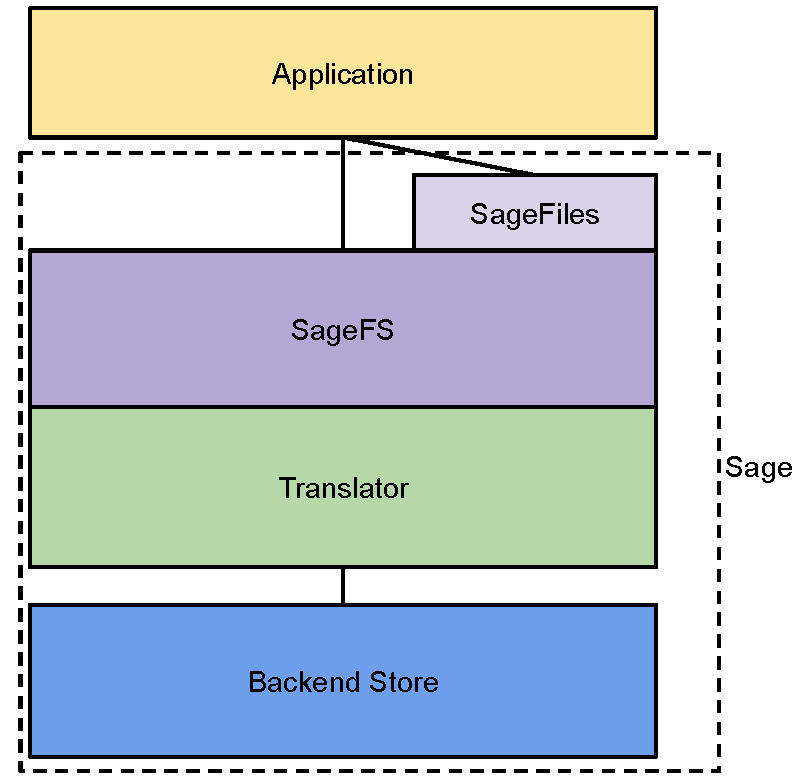
\includegraphics[scale=0.7]{figures/archetecture}
\caption[Sage Archetecture]{Sage Archetecture.}
\label{fig:archetecture}
\end{figure}

An application sees Sage as one filesystem, where within Sage many translators may exist connecting to many different backends. To do this applications interact with SageFS to perform filesystem operations like listing, opening, or removing files, and interact with SageFiles for individual file operations like reading and writing. SageFiles behave exactly like normal files opened normally through the operating system with one exception. They hold Sage specific metadata which allows Sage to place the file in the correct backend using the appropriate translator. SageFiles only interact with SageFS, not translators; this means Sage can move SageFiles between translators without the file knowing. Sage can then move files easily inbetween backends as shown in Figure \ref{fig:sagecommunication}.

SageFS is the only component that interacts with the various translators. Internally SageFS holds a collection of translators. When an application makes a Sage filesystem call, SageFS selects the appropriate translator and forwards the request. This approach lets us define an API for SageFS, which is then implemented by the translators. The Sage API currently contains seven methods open(), remove(), list(), stat(), copy(), move(), and upload(). A translator must implement all seven API calls and convert them into the appropriate set of backend calls. A translator is connected to exactly one backend. The open() call retrieves file data from the connected backend store and returns it in a SageFile. It is also used to create a new file. The remove() call removes file data while list() lists all files present in the backend. stat() returns file metadata such as size, copy() duplicates a files contents, and move() moves a file around in the backend store. The actual implementation by the various currently implemented translators is discussed in Chapter \ref{chapter:imp}.

\begin{figure}[h!]
\centering
%keepaspectratio=true, width=\textwidth
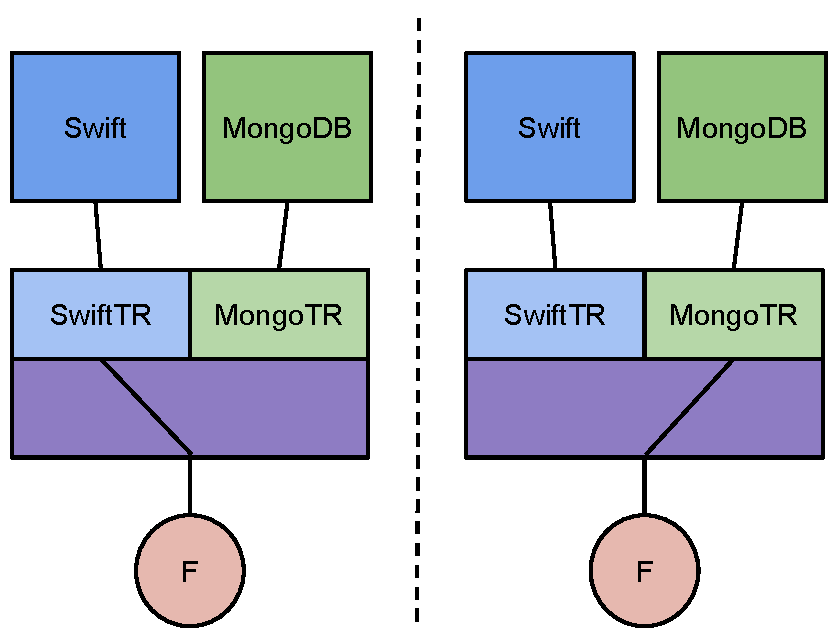
\includegraphics[scale=0.7]{figures/sagecommunication}
\caption[File Interaction in Sage]{File Interaction in Sage. On the left the file F is stored in Swift. SageFS (purple) forwards file requests to the SwiftTR translator. On the right F is stored in MongoDB.}
\label{fig:sagecommunication}
\end{figure}


\section{SageFS}

SageFS creates a common API to many backends systems, but also integrates the backends to look like a single filesystem. SageFS holds a collection of translators that convert filesystem commands into the appropriate set of backend commands. Filesystem commands are performed on paths just like in a posix system, where the root of the path maps to a translator (here we consider \textit{``''} an empty path). For clarity let's examine what happens when an application calls open() on the path \textit{``/vic/test.txt''}. SageFS considers the root to be everything from the leading slash to the second slash of the path, which in this case is \textit{``vic''}. SageFS then maps the root to a translator and calls the translators open with the remaining path, namely \textit{``test.txt''}. Of course, the path could be much larger with many directories. It is the translator's job to map the remaining path to the appropriate data in the backend. In this sense, one of the translator's main functions is to act as a name server for the backend storage service.

List and stat are the only commands that take the empty path as a valid argument. If we look at list, it normally takes a directory as an argument, which prompts SageFS to call the appropriate translators list. However, with no argument SageFS will call list on all the translators it knows about, returning a list of all files within the filesystem. Stat performs the same way.

From the above example it may become clear that Sage knows nothing about which backend files belong to initially. In fact, all file metadata is stored with the backend store. This allows Sage to avoid consistency issues where a backend and Sage disagree on the state of a file. Furthermore, this allows the backend to be manipulated through other channels of operation (not through Sage) without interfering with Sage itself. It also allows multiple Sage instances to connect to the same backends and not have to know about one another. As an aside, all current Sage backends use REST calls to communicate. A backend requiring a constant connection should behave the same way as a REST based one, but this has not been attempted within Sage.

An instance of Sage is a collection of translators that communicate with backend storage services. A single translator talks to a single backend, so if for example we have two backend stores both using Swift, we need two translators one for each Swift instance. We do this as each translator must be independently addressable. If we want to take advantage of each Swift instance independently, we need a way to differentiate between the two. The way Sage holds translators also allows us to add and remove backends by modifying the set of translators in the Sage instance. In fact, when a Sage instance is initially instantiated, the set of translators is empty! It gets populated during operation as backends are addressed. Although more of an implementation detail to reduce initialization time, it demonstrates how resources can be added on the fly to Sage by manipulating the set of translators.

Applications can take advantage of the translator set by explicitly requesting certain backends via the path. By doing this applications can choose where files are placed within Sage. Having control over file placement is beneficial to applications where file location matters, but many applications do not care where their files are placed. Sage can determine file placement if the application does not, and does so through a file placement function. This function takes a full file path and returns a translator within Sage, which is forwarded the request. The default file placement function is primitive. It simply randomly chooses a translator to return, but applications can overwrite the default. Figure \ref{fig:fileplacement} shows the interaction between an application, Sage, and the file placement function. The file placement function can be defined by an application and used to write custom file placement logic.


\begin{figure}[h!]
\centering
%keepaspectratio=true, width=\textwidth
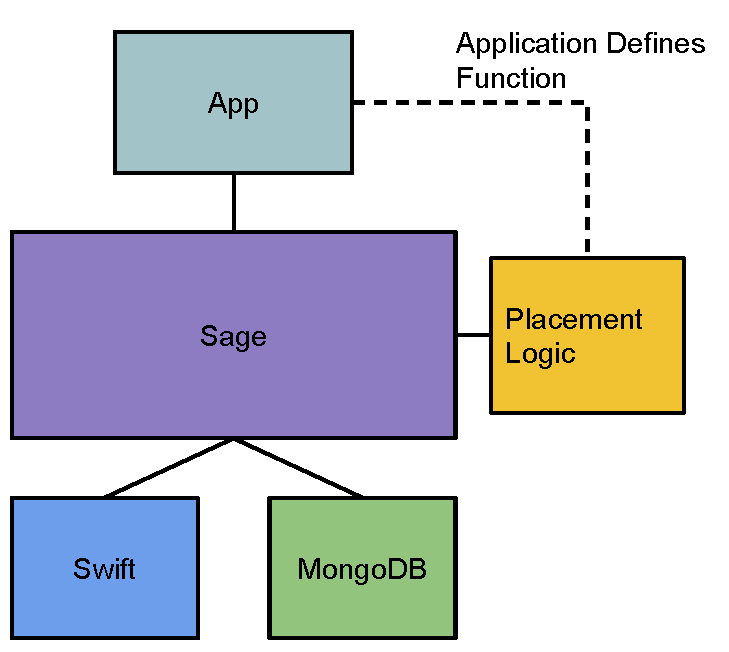
\includegraphics[scale=0.7]{figures/fileplacement}
\caption[Sage File Placement Component]{Sage File Placement Component. Applications can supply a function to overwrite the default file placement logic in Sage.}
\label{fig:fileplacement}
\end{figure}


\section{Filesystem Concepts}

In this section we examine common distributed filesystem concepts, and how they look within Sage.

\subsection{Caching}

Distributed filesystems normally have some form of caching mechanism on clients. Caching helps improve overall performance by providing local copies of resources, so clients do not constantly have to contact storage devices. Sage translators cache file data when a given file is opened within an application. Data is pushed to the backend store when the open file is written to or the closed in Sage. A file is only pulled from the backend when it is opened within Sage, so to revalidate a cached file, the file must first be closed then reopened. More aggressive caching could be performed, where a set of files is kept locally even after they are closed. To do this a timestamp would have to be stored along with the file that could be used to check for staleness by asking the backend store when the cached file was last updated using the stat command.

Sage has no form of cache invalidation. If a stale file is modified on a client and written back to the storage device, the modified stale file will be the authoritative copy of the file. Again Sage could check for timestamps using stat, however a race condition exists here. Suppose we have two clients A and B that want to write a file in the same backend. Client A asks the backend for the time the file was last modified. At the same time Client B asks the backend for a timestamp as well. The backend processes both requests and returns the same timestamp. A and B conclude the file is safe to write when there is a conflict, and the last write will win. This problem comes from a lack of atomicity in the timestamp request. A client can not assume the file has not been modified in the time it takes to get the timestamp from the backend. File locking is normally used to avoid this issue which Sage leaves this up to the backend to handle. If a backend store uses file locking then the translator using the backend will also have file locking, however Sage makes no guarantees about locking in general.


\subsection{File Locking}

As we previously saw, file locking is a way to ensure file consistency with concurrent access. In Sage file locks would either have to be given out by backend stores or each client would have to be aware of each other client and synchronize locking between them. The latter solution is unattractive as clients are allowed to change networks, be behind NAT routers, or perform any other mischief that a traditional network connection would dislike. Furthermore, the filesystem namespace is unique to each client, which would require translation to a common namespace between clients. Moreover, if above problems were not enough of a deterrent the actual locking process would be much worse. 

Clients could hold locks for files but must check first if any other client had a lock on the same file. In the ideal case we, a client, request a file lock and get replies from all others saying they do not have a lock on the specified file. However, what happens if a client does not reply? Do we assume the unresponsive client does or does not have a lock? If the former then we could be waiting for the lock for a while, if the latter then the unresponsive client could assume it has the only lock and commit conflicting changes to the filesystem. Furthermore what if during our lock request we get a request from another client for a lock on the same file. In this case who takes the lock? If we back off and try again (with a random back off or similar strategy), we could potentially get into livelock where we are constantly waiting for locks. This is essentially an instance of the Byzantine Generals problem \cite{Lamport1980,Lamport1983}. Distributed clients must agree on some value (the lock in this case), in an environment with Byzantine failures. Unfortunately, the problem is unsolvable if one-third of the clients fail as consensus requires at least $n/2 + 1$ clients to agree on the value.

Distributed locking is extremely difficult and in fact most distributed lock managers use a central component to avoid such issues. Locking is left to backends in Sage for those reasons. Translators decide how to handle locked files and locks. Since the open call in Sage takes optional arguments locking parameters could be passed into Translators to request locks either blocking or nonblocking. Locks would persist until the file is closed within Sage unless some modification to the API were made, or the application interacted directly with the Translator.

One other issue to consider with locking is Deadlock. Deadlock is a hard issue and normally handled by having locking orders, or by some detection mechanism. Unfortunately in Sage locking orders would be difficult to implement as each client could have a different collection of backends (or the same collection with different names). Hostnames could be used to create a lock order. This way clients get locks from the lexicographically least host first. However, backends can use proxy servers so clients could potentially interact with different hosts to access the same backend. Distributed deadlock detection can be used to track down deadlocks while the system is running by constructing a wait-for-graph \cite{Haas1983}. A wait-for-graph is built between nodes by tracking lock requests and adding edges between nodes that are currently waiting for another. Deadlocks are represented by cycles in the graph. Unfortunately, the graph has to be built at a central component and requires knowledge of all nodes in the system.

Clearly locking poses many problems within the architecture of Sage and is why it is left to the backends. Not only does it simplify the architecture but it also makes Sage more flexible as a system, two key design goals of Sage.


\subsection{Metadata Management}

In Sage metadata is stored with files, much like in a normal filesystem. Filesystem metadata is either stored in the client or queried from the backends. Normally filesystem metadata is stored in a central server, or distributed over a few metadata servers (known as MDSs). With a central MDS, the system has a single point of failure, however with distributed metadata we need to make sure the metadata remains consistent. Sage does not maintain metadata as its flexibility allows backends to be added on the fly which would require a merging of metadata if one were added. Additionally backends can be modified out of band, which could result in files being deleted or modified without the MDS knowing and inconsistencies in the system.


\subsection{Replication}

Replication is usually done in distributed filesystems to improve availability of files. Files are replicated to allow concurrent access,  improve locality, or increase durability. If a file is replicated to multiple copies, updates must propagate to all copies or applications may see inconsistent data (and may modify the inconsistent copy). To enforce consistency systems usually opt for either weak or strong consistency models. Weak or eventual consistency as it is sometimes called guarantees consistency throughout the system eventually. Updates are propagated throughout the system and processed asynchronously by nodes. Operation is not stopped so applications can potentially see stale data if their request is handled before the update. For many applications this is good enough. However some need a better guarantee of consistency. Strong consistency guarantees that once a change is committed, all copies will have the change applied before other applications can access them. This is useful if applications need up to date data, such as a filesystem. It does however impact availability as replicas will be unavailable while a change is being applied.

Keeping the above two schemes in mind Sage could implement replication by assigning replication groups within the client. A replication group is a collection of translators that would perform the same file operations in parallel when one of the members is accessed within Sage. For example, imagine we have a collection of six translators (1 $\dots$ 6). We can set up replication groups as subsets of the translator collection with group size according to the replication factor. With a factor of three we can set up groups (1,2,3), (4,5,6). When a file is accessed through translator 1, it can be read normally, however when changes are made the file is pushed back through translators 2 and 3 as well. This way if translator 1 fails, copies are still on 2 and 3. Updates are done in parallel and should only succeed if updates to all the translators succeed. This is a form of strong consistency as updates are done to all copies and only committed if all replications are updated. There is one caveat here; no file locking is done so it would be possible for two copies to be updated at the same time and writes to overlap differently at different locations. As an illustration assume a file is modified at two places and pushed to the translator group (1,2,3) at the same time. Since last write wins, whichever request is process last is the definitive version of the file. However, each backend could receive modifications in any order and therefore the last update could be different at different nodes. The pushes would succeed, but the file may be inconsistent. Replication groups would have to be the same over all clients or implemented inside translators as clients should know about all replicas of a file to avoid updating only a fraction of the file replicas.

The lack of a dedicated metadata server means replica placement must be computable by a client. Sage could also use hashing to distribute replicas via a consistent hashing algorithm such as CRUSH (previously seen in Chapter \ref{chapter:rel_work}). A filename could be hashed to produce a set of backends to replicate the file to. The set of backends again benefit from being static as adding new backends requires files to be rebalanced to their new hash values. This would involve moving many files between backends, would have to be done by the clients, and cause significant overhead in the filesystem.

\section{Considerations}

Many of the systems currently left to the backends could be implemented if filesystems could not be changed on the fly and were defined for all clients. A static Sage deployment could implement some of the systems discussed. Some design ideas in this chapter could make logical starting points for an implementation, but no prototypes have been developed. The next chapter presents the implementation of Sage. Further discussion of some of the features and ideas presented here are addressed in Chapter \ref{chapter:conc}.
	\startchapter{Implementation}
\label{chapter:imp}

In this chapter we take a look at how the Sage prototype is implemented. We
examine each  filesystem object in detail and finally look at how Sage is
actually used.

\section{Overview}

\note{Users and groups??? Gotta talk about it somewhere as i do a bit in future work}

SageFS (or Sage) is implemented as a Python client library and is used by
importing into a  Python project. I chose to use a client library instead of
system component was because a  client library is much easier to use and
deploy. Additionally the initial use case for  Sage was for Python
applications accessing a large repository of satellite imagery as discussed in
the Green  Cities application in Chapter \ref{chapter:intro}.  Once imported,
a Sage object can be created to interact with SageFS, which contains a number
of translator objects. Currently there are only two types of translators,
SwiftTr and MongoTr  that connect with Swift object stores and MongoDB
instances respectively. Translators are the components that actually interact
with backend stores, and essentially translate filesystem  commands into the
appropriate set of commands for the backend storage. For example, when the
SageTr object's open method is called on a file in a Swift backend, SageFS
call the containing  SwiftFS open which downloads the file and stores it in a
SageFile object for use by the application.  SageFile objects are file
abstractions built on top of Python files. SageFile objects have two
subclasses, namely SageMemFile and SageDiskFile objects. Both have the same
functionality, however  SageMemFile objects exist in memory only, while
SageDiskFile objects are actually written to disk.  Applications communicate
with SageFS directly and through the use of SageFiles. To store files in
backend repositories SageFS communicates with translator objects, notably
SwiftTr and MongoTr  which actually communicate back to the backend. This way
Sage can make multiple backends appear  as a single entity, with a common API.

One important thing to notice here is that Sage does not go through the OS for
normal operation.  The OS is used for networking and to put opened files on
disk (if they are requested not to  reside in memory). However, if a
translator does not go through the OS, an application that  used the `no OS
translator' could use normal Python file operations and never go through the
OS!

\begin{figure}[h]
\centering
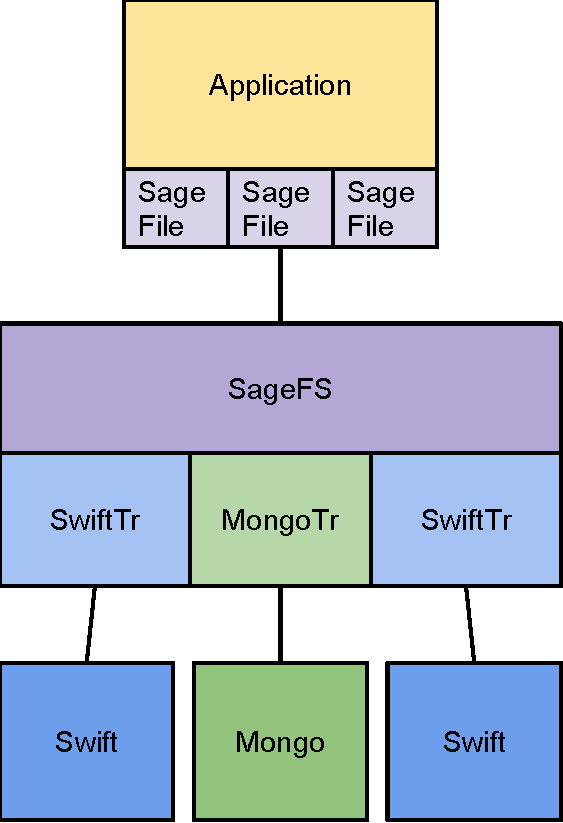
\includegraphics[scale=0.7]{figures/implementation}
\caption[Example Sage Deployment]{An Example of a possible Sage deployment with the current Implementation}
\label{fig:implementation}
\end{figure}


\section{File Objects}

We start looking at the filesystem by examining the actual file objects.
There are two types of Sage file objects, SageMemFile and SageDiskFile.  Both
objects inherit from the SageFile class, but SageMemFile inherits from  the
StringIO class while the SageDiskFile inherits from the base Python file
class. This allows the SageMemFile to reside as a buffer in memory, excellent
for smaller files that are consumed rapidly and do not need to be persisted,
while a SageDiskFile is actually written as a temporary file on the client
system.  The base SageFile object has a few key variables and methods that
facilitate interaction  with Sage. Each SageFile knows which backend
repository it belong to and uses this  in the sync() method which re uploads
the file into the backend. sync() can be called  on its own but it is also
called within the write() family of methods for SageFile  objects. If we take
the write method as an example, we see it takes three arguments.  The first is
a reference to the calling object (Python makes this explicit, while in  a
language like Java the self reference `this' is always the first argument to a
method,  but not explicitly stated in the method signature). The second
argument is the argument  to the underlying file object's write method, while
the third is a flag indicating whether  or not we should sync the file at the
end of the write operation. This is included incase  we only want to update
the local copy and not write back into the backend repository after  every
write (ie. cached writes). The close() method looks similar to write() except
it only  takes the sync argument. When a file is closed it is first synced
back to its backend  repository, then removed from a local filesystem cache
from sage. The file is only removed  if the sync was successful so If an error
occurs, the file will still reside in sage and no  data is lost. A special
method for SageFiles called todisk() will take the file from Sage  and persist
it to the local system. This is a convenience method that allows files to be
easily taken from Sage.

\begin{figure}[h]
\centering
\begin{lstlisting}

def write(self, arg, sync=True):
  """ Calls the underlying write function for the file.
  Will sync with remote storage by default, 
  will not if sync is False """
  self.fileclass.write(self, arg)
  if sync: self.sync()

\end{lstlisting}
\caption{SageFile write function}
\label{fig:sagefilewrite}
\end{figure}

\begin{figure}[h]
\centering
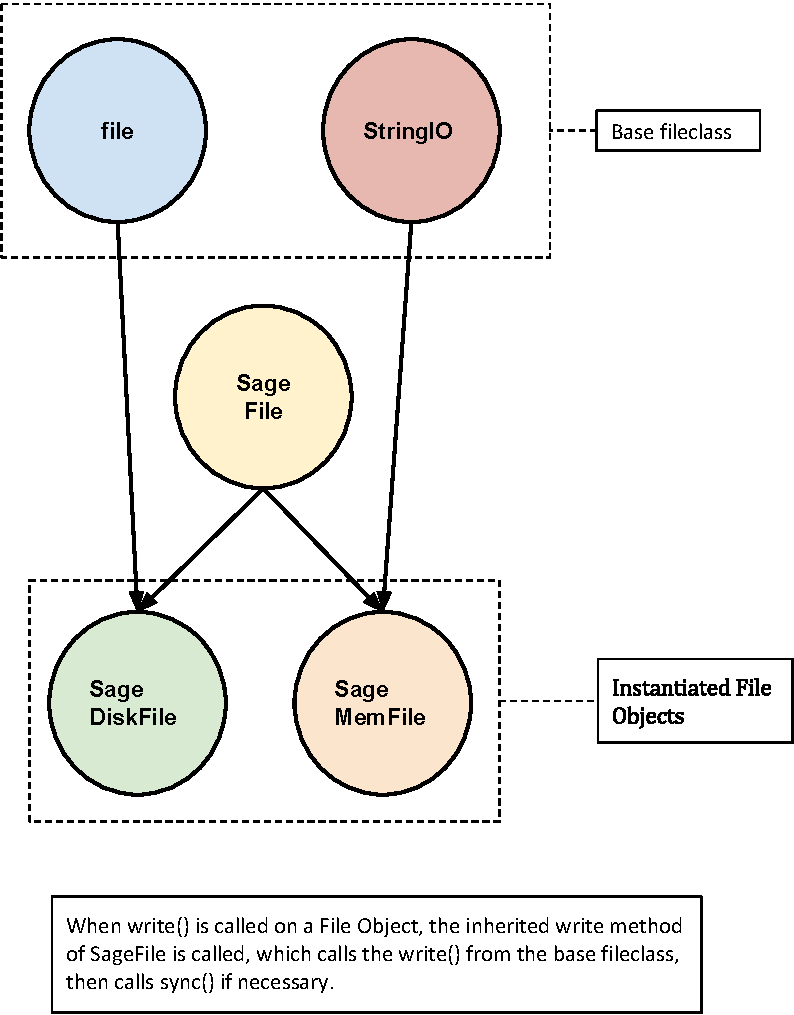
\includegraphics[scale=0.7]{figures/sagefile}
\caption{SageFile inheritance graph}
\label{fig:sagefile}
\end{figure}


\section{Backends}
\label{sec:backends}

Before we examine translator objects lets first take a look at the backend stores that
FS objects actually connect to, and how we can view them as filesystems.

\subsection{Swift}

Swift is an object store system developed by OpenStack as an open source
alternative to Amazon's S3. Clients interact with Swift's RESTful api through
HTTP using PUT and GET to access files. Swift has two main types of nodes,
storage which actually store data, and proxies which handle requests to Swift.
What makes a machine a storage or proxy node depends on the set of processes
running, and in fact a single machine can be both a storage node and a proxy
node. Swift distributes and replicates files across all storage nodes using
what are called `rings'. Figure \ref{fig:swift} shows an object placed
within a Swift cluster. When an object is stored in Swift it is first assigned
to ring, which then handles distribution over a set of storage nodes where it
is stored as a blob. The Proxy node handles the partitioning of the file based
on the ring configuration, then sends data to the storage nodes. The number of
nodes a file is distributed to is called the replication factor for the
storage set. It is worth noting that all requests go through the proxy nodes
(a cluster can have multiple proxies and each request goes to exactly one of
them), so clients never directly contact the storage nodes.

\begin{figure}[h]
\centering
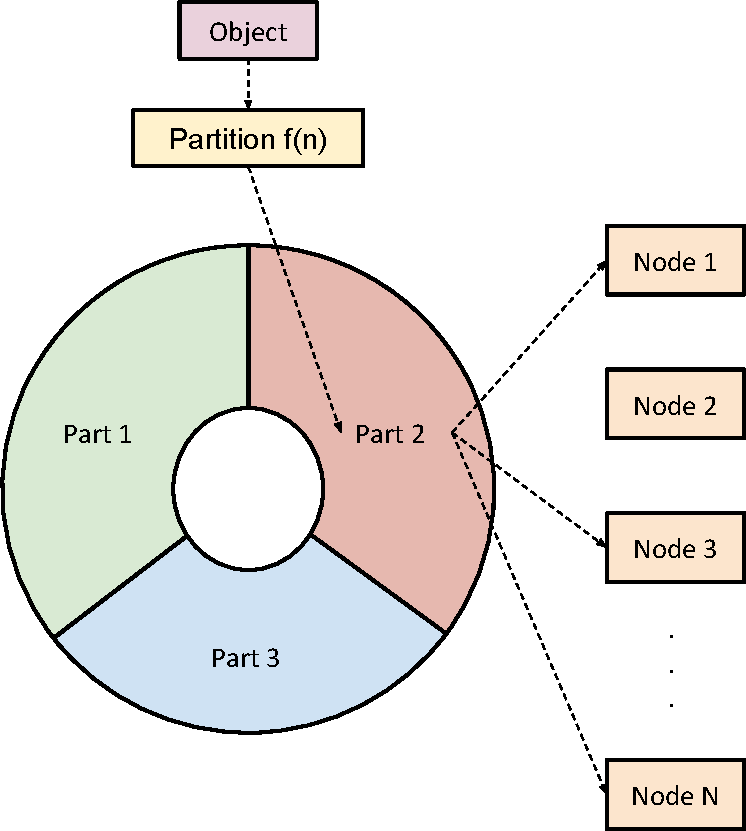
\includegraphics[scale=0.7]{figures/swiftrings}
\caption{The OpenStack Swift Ring Structure}
\label{fig:swift}
\end{figure}

Swift also contains accounts and containers which logically separate files
into groups which I use to implement users and groups in Sage. Each group is
an account and each container is a different user. We could have easily
implemented an account for each user since groups are not implemented in the
filesystem, but using accounts is one way future implementations could. Files
are stored based on their full path so directories do not physically exist,
though Swift can mark a zero byte file to act as a directory. The Swift client
allows partial name matching which we can use to search for all files
logically grouped in a directory by simply querying the path name as a
substring. We use the swiftclient module to communicate with Swift through
Python.

\note{put\_object and get\_object? Also the figure of how users and groups are done}


\subsection{MongoDB}

MongoDB is a NoSql database which stores objects in what is called document
oriented storage. Related documents are organized into collections that allow
efficient querying and indexing. Data is stored as BSON a superset of JSON
that allows Mongo to store arbitrary bytes of data. Mongo can exist as a
standalone database on one machine, or can be distributed in a cluster. When
distributed Mongo has Config Servers which hold metadata, and Shards that
house the data. A given document collection can be distributed across shards
much like disk striping. Config Server metadata is held in a config database
(a single Mongo instance can contain multiple databases) which maps documents
to Shards. Shards contact the Config Servers to access metadata (which Shards
heavily cache). I make use of databases and collections to implement users and
groups, and store files as a key value pair document, with the key being the
full file path, and the value being the files binary data. In the actual
document we store path and file name as two separate fields as we want to be
able to search for paths and partial paths when listing files. We use the
Python module pymongo to communicate with MongoDB.

\note{collection.insert and collection.find\_one ????}


\subsection{Local}

A very rough implementation exists to incorporate the local filesystem into
Sage. This was developed mostly for testing purposes and is missing
functionality other than reading and writing files. Files are created in a
temp directory which acts as the root for the filesystem.


\section{Translator Objects}

Translator objects in general must implement upload() open() stat() copy()
move() list() and remove() methods as SageFS hands off functionality to the
translator objects when performing filesystem operations. Additionally the
translator must keep a list of files opened with it that have not been closed.
The open() call is one of the only calls that can change the state of the
filesystem as it opens a file descriptor within the system. open() is actually
called on the SageFS object which then calls the underlying translators open()
passing the arguments through. We visit the SageFS object later in the
section. As we can see from the method signature in Figure \ref{fig:sagefsopen}
the open() call has one required parameter and two optional, create which
defaults to false and inmem which defaults true. If the file specified at path
does not exists in the repository and create is true then an empty file will
be created for the translator to keep track of. The file is not actually
created in the backend until it's sync() method is called. The second argument
specifies whether the file should reside in memory or on disk on the local
system. If inmem is true then the file is opened as an SageMemFile, otherwise
it is opened as a SageDiskFile. If open is called on an already open file, the
translator returns the open file descriptor for the file instead of a new file
descriptor for the file. This is done to avoid consistency issues to do with
having two sets of the same file downloaded. It would be possible to implement
file pointers within the SageFile object to allow having two file descriptors
for the same file, but this functionality does not exist in the current
implementation.


\begin{figure}[h]
\begin{lstlisting}

def open(self, path, create=False, inmem=True, *args):

\end{lstlisting}
\caption{The SageFS API's open method signature}
\label{fig:sagefsopen}
\end{figure}

The rest of the translator is convenience methods or methods for connecting to
the backend repository. For example SwiftFS is an object that holds all the
relevant info to connect to swift as well as interface back with SageFS. The
actual Swift repository knows nothing about the front end translator and
communicates via the RESTful interface provided. This makes implementing translators
simple since the six methods just have to be translated into the appropriate
REST calls. The translator also converts filesystem paths into actual
locations in the backend store. Since both Swift and MongoDB are not natural
filesystems we have to fake paths and folders within them. To do this we
simply incorporate the full path as the actual name of the file in the backend
store. This allows the filesystem to logically separate files into a virtual
directory tree, and query based on a fragment of the path. Both Swift and
MongoDB have partial querying built in, but if a backend store was used that
did not have such functionality, then the translator would have to query every
file in the backend and filter the results in the client which could have a
large performance impact.


\section{SageFS}

The SageFS object is the central component of the filesystem and implements
the API (the seven methods  open(), remove(), list(), stat(), copy(), move(),
and upload()) exported for use by applications. Of course an application could
use any part of the sagefs.py Python module, but the intended use is to
interact with the SageFS object. The SageFS object holds a dictionary mapping
names to translator objects as well as a list of all the available backend
repositories, called sites, to the Sage instance. The SageFS constructer and
connect\_to\_filesystem methods are shown in Figure \ref{fig:sagefscode}. The
actual translator objects are not instantiated until the site is actually
used. When a site is accessed the connect\_to\_filesystem() method is called
which creates an translator object and stores the object in the filesystems
dictionary. If more backends were to be added the connect\_to\_filesystem()
method would need to be modified to handle creation of the filesystem objects,
and the constructor for SageFS would need to store a new list for the new
backend repository type. This approach is not the most scaleable so if many
new types of filesystems were to be added, the constructor should take a
dictionary of site names and the constructor method of the appropriate
backend. This way connect\_to\_filesystem() can index into the new dictionary
and call the translator constructor without going through a long chain of
if/else statements.


\begin{figure}[h]
\begin{lstlisting}

class SageFS():
  """ The main filesystem object which holds a collection of SwiftFS
  and MongoFS objects. Connections are only established when they
  are used the first time. The SageFS object is designed to be the 
  only object that must be explicitly created to use the SageFS. """

  def __init__(self, swiftrepos=hosts.swift, mongorepos=hosts.mongo):
    self.filesystems = {}
    self.swiftrepos = swiftrepos
    self.mongorepos = mongorepos
    self.sites = self.swiftrepos.keys() + self.mongorepos.keys()

  def connect_to_filesystem(self, site):
    """ Creates a translator object if we correctly connected """
    fs = None
    if site in self.swiftrepos.keys():
      repo = self.swiftrepos[site]
      fs = SwiftFS(repo.get_authv1_url(), repo.group, repo.user, repo.key)
    elif site in self.mongorepos.keys():
      repo = self.mongorepos[site]
      fs = MongoFS(repo.host, repo.port, repo.database, repo.collection)
    else: raise SageFSException('No host matches site %s' % (site))
    self.filesystems[site] = fs
    return fs

\end{lstlisting}
\caption[SageFS Constructor]{The SageFS constructor and connect\_to\_filesystem methods. The class instance variable self.filesystems holds the SageFS objects collection of translators.}
\label{fig:sagefscode}
\end{figure}


From a high level, when a method is called on the SageFS object the method
first chooses the correct translator based on the file placement logic, then calls the
underlying translators method to perform the call. In the current stable
implementation of placement logic is done by path name via the method
split\_location\_from\_path() (which is easily extended as discussed in section
\ref{chapter:conc}). The method returns an index into SageFSs filesystem
dictionary, which is then used to grab the appropriate translator to perform the
operation on. Some operations operate over a set of translators, stat() and list() can
be used to probe all the translators, while copy and move may involve two different
filesystems. To get a better understanding of how the components work together
in SageFS let us examine the copy() method, shown in Figure \ref{fig:sagecopy}, as while it is the most
complicated, it demonstrates the power of the aggregation of multiple translators in
SageFS.

\begin{figure}[h]
\begin{lstlisting}

def copy(self, origpath, newpath, overwrite=False):
  """ Copy a file from 'origpath' to 'newpath'.
  Will not overwrite unless specified """
  if origpath == newpath: return
  origlocation, origresource = self.split_location_from_path(origpath)
  newlocation, newresource = self.split_location_from_path(newpath)
  origfs = self.get_filesystem(origlocation)
  if origlocation == newlocation:
    # if both resources use the same fs use the fs's copy
    origfs.copy(origresource, newresource, overwrite)
    return
  newfs = self.get_filesystem(newlocation)
  # check to see if we are overwriting anything
  if not overwrite and newfs.file_exists(newresource):
    raise SageFSFileExistsException('File %s already exists' % (newpath))
  local = True
  if origresource not in origfs.localfiles:
    # make sure the orig file is local to its fs
    local = False
    origfs.open(origresource)
  origfd = origfs.localfiles[origresource]
  # upload as a new resource
  try: newfs.upload(newresource, origfd)
  except swiftclient.client.ClientException as e:
    raise SageFSException('HTTP Error: %s - %s' 
               % (e.http_status, e.http_reason))
  if not local: origfd.close() 

\end{lstlisting}
\caption{The SageFS API copy method}
\label{fig:sagecopy}
\end{figure}

The method takes three arguments, origpath which is the path to the original
file to copy, newpath which is the desired path to the new copy of the file,
and an optional argument overwrite which specifies whether the newpath should
overwrite an existing file if it exists. First the method checks if we are
trying to copy to the same location to avoid redundant work, if we actually
need to copy then we determine which filesystems the old file and new file
belong to (or should belong to). If the copies will reside in the same
filesystem we then delegate the work to be done by the translator object, and pass
along the arguments. If they will not reside in the same translator we first check if
we should overwrite the new location and if so, that a file does not exist at
that location. If either of the above is true then we raise an exception
saying that the file already exists. Next we check to see if the SageFile is
open in the original files translator. If it does not then we must open the file so we
can copy it and we also want to remember the file was not open at the start of
the call so we set the variable local to false. We then call upload on the new
translator, giving the new file name and the old files data as arguments. This makes a
copy of the file in the new filesystem without actually opening the file which
ensures the set of open files in the new translator remains unchanged. We finally
close the original file if it was not local to the original translator as again we
want the set of open files to remain unchanged.


\section{Configuration}

SageFS takes a collection of repositories as arguments, which can either be
passed to the constructor or defined in the configuration file hosts.py in the
sagefs python package. The configuration is a dictionary of Host objects in
this case SwiftHosts and MongoHosts. These objects define connection
parameters to each of the backends including username, hostname, and the key
which will identify the filesystem. As an example Figure \ref{fig:swiftconfig}
shows a configuration dictionary for Swift filesystems and is the dictionary
that is passed by default to the SageFS constructor shown in Figure
\ref{fig:sagecode}. The dictionary contains three entries vic, tor, and carl that
map to three SwiftHost objects which simply define parameters to connect to a
Swift repository. Here we see the IP addresses of three Swift installations
that are used as backends and are actually used in the deployment of SageFS
for the genome searching case study described in Chapter \ref{chapter:exp}. To
add or remove filesystems to Sage the we can simply modify the dictionaries in
the configuration file with the appropriate connection parameters, or simply
pass in our own dictionary to a SageFS object.


\begin{figure}[h]
\begin{lstlisting}

swift = {
  'vic':SwiftHost('142.104.17.135', 'admin', 'system', 'sagefs'),
  'tor':SwiftHost('142.150.208.220', 'admin', 'system', 'sagefs'),
  'carl':SwiftHost('134.117.57.138', 'admin', 'system', 'sagefs')
}

\end{lstlisting}
\caption{Configuration dictionary for Swift backends}
\label{fig:swiftconfig}
\end{figure}

Currently, the SwiftHost and MongoHost objects are the only SageHost objects
defined in hosts.py. SwiftHosts require a hostname (or IP address), user,
group, and key to connect to a Swift backend, while MongoHosts require a
hostname, database name, and collection name. Section \ref{sec:backends}


\section{Using Sage}

To use Sage from a client perspective we only needs to import the sagefs
Python module into their Python project. This will allow us to use SageFS with
the default filesystems and defult user provided in the hosts.py configuration
file. To use different filesystems we can either modify hosts.py or pass in
our own dictionary containing the desired filesystems. One thing to note is
that if we define a filesystem that does not exist or does not accept the
connection parameters we provided, SageFS will not fail until we try and
access the dysfunctional filesystem. We can also define a filesystem twice
with a different dictionary key. SageFS will think the two filesystems are
different and allow file operations on both. If we open the same file in both
filesystems two copies of the same file will exist on our machine and if we
write different things to each copy, the copy with the last sync() operation
will be what appears in the backend (If the backend has no file locking!).
This implies that SageFS does no file locking and leaves it up to the backend
store as discussed in Chapter \ref{chapter:arch}.

\begin{figure}[h]
\begin{lstlisting}

import sagefs
fs = sagefs.SageFS()
__builtins__.open = fs.open

\end{lstlisting}
\caption[SageFS Open Hack]{An interesting hack to overwrite Pythons builtin open call to use Sage's instead.}
\label{fig:sagepythonhack}
\end{figure}

Once the module has been imported we create a SageFS object which allows us to
perform operations on the filesystem. To interact with files we call the
SageFS objects open() which returns a SageFile object, which is then used
normally like any other Python file object. In fact if we were to modify an
existing python project to use Sage we would only need to import the sagefs
module, then instantiate a global filesystem object and overwrite the built in
open() function with our filesystems open(). After doing this all calls to
open will go through Sage and all file objects will be SageFiles and will work
without further modification. We could also go a step further and define a
closure around Sages open to extract information about the file and pass it to
open() to allow interesting file placements! Of course other operations from
other modules that utilize the built in open() or modules that manipulate the
local filesystem will remain unchanged so more work may be required on a more
complicated system. Additionally Sages open() will throw different exceptions
than the built in so applications would suffer from unexpected errors if one
occurred.

The client side of SageFS is implemented as a python package which can be
downloaded from github. I also developed server side deployment scripts for
Swift, which will install and configure Swift on a cluster of machines (either
Ubuntu or Fedora) using the Fabric Python module. Once the Swift cluster (or
clusters) are running, the hosts.py file can be edited to make the clusters
the default filesystems, or we can pass the appropreate dictionary to our
SageFS object.

	\startchapter{Experiments and Evaluation}
\label{chapter:exp}

%\section{Overview}

In this Chapter we examine the performance of Sage as well as how Sage performs in terms of the design goals. Specifically we look at the overhead of filesystem calls from within Sage versus performing the same calls outside of Sage. File reads and writes are measured to see the overhead on file operations, and file lists, removes, and creates are measured to see the overhead on filesystem operations. All measurements are made with the current implementation using two backends Swift and MongoDB. The experiments use the same data schema for Swift. The directory heirarchy is implied by the stored object names in Swift. For MongoDB however the schemas are slightly different. Going directly to MongoDB files are stored as \textit{fullpath:data} pairs, while going through Sage to MongoDB files are stored as \textit{path:filename:data}. I do this as the most natural way to store files in MongoDB is to use \textit{fullpath:data}, so going directly to the backend uses that schema. The translator does not as I wanted to make paths queryable within the translator. This implementation detail reinforces the fact that the translator implementation makes a difference to the filesystem performance as we will see later in the chapter. Finally, all microbenchmark experiments were performed on Emulab as I wanted the results to be as reproducible as possible \cite{emulab}.

After the microbenchmarks we then look at a case study of an application using Sage to perform analysis on human and viral genomes, specifically looking at how an application can take advantage of file placement within Sage. Finally, we conclude with an examination of types of applications that could take advantage of what Sage offers, and those that would be better off using a different system.

In the spirit of reproducibility, all the benchmarks are scripted and can be found at \url{https://github.com/stredger/sagebench}, while the case study can be found at \url{https://github.com/stredger/dnasearch}. Scatterplots for all data presented in this section can be found in Appendix \ref{chapter:appendix}.


\section{Microbenchmarks}
\label{sec:microbench}

I ran microbenchmarks on the Emulab computing platform using an Ubuntu12 64-bit OS image. Emulab allows us to run on bare metal, not inside a VM so we can ignore any artifacts a VM may produce. I wanted to see how much overhead was incurred by going through Sage instead of directly accessing files from their respective backends. Additionally I wanted to see the differences between the two implemented backends Swift and MondoDB. Both MongoDB and Swift were set up on the Emulab experiment nodes. Mongo used a single node configuration while Swift had one proxy node and one storage node. Swift needed two nodes as using a single node for both storage and proxy, two components Swift requires, was causing crashes when running the larger tests. For these microbenchmarks, I used Emulabs d710 machines that are 64-bit and have 2GB of memory.

I ran tests by writing a simple Python script that performed file uploads and downloads using the sync() and open() calls from SageFS. The put\_object() and get\_object() calls were used from the swiftclient Python module to measure interaction with Swift, and db.collection.insert() and db.collection.find\_one() from the pymongo module to interact with MongoDB. These library calls are used internally by Sage so are used to measure time to go through the module versus the time to go through Sage. Timestamps are taken just before a call and just after it returns. Timestamps are stored in a list that is written to disk after the experiment has completed. 

I ran each test 100 times for a range of file sizes 1KB, 10KB, 100KB, 1MB, and 10MB. I also attempted to run a 100MB test, but unfortunately MongoDB imposes an arbitrary file size limit of 16MB so I did not run the 100MB test using the MongoDB backend. I could have split up the file into smaller chunks, and in fact this is what MongoDB recommends for large files. However, I made the decision not to perform the test as normal usage in this case is to upload ten 10MB files, which is simply the 10MB file test with more runs.

The Emulab nodes had a small disk size, so the 100MB tests were performed slightly differently. The hundred iterations were split up into runs of ten. A run uploaded ten files, then deleted them to free up disk space so the next run could proceed. 

The platforms I measured were Swift, MongoDB, Sage using a Swift backend, Sage using a MongoDB backend, and the local disk. I chose these to look at the performance overhead of going through Sage compared to Swift and Mongo. The local disk is used as a measuring stick to put the measurements into context.


\input chapters/5/table.tex

Tables \ref{tab:microput} and \ref{tab:microget} summarize the micro
benchmark test results for all file sizes and backend stores. All times reported in the tables are in milliseconds.



\subsection{File Put Benchmarks}

\begin{figure}[h]
\centering
\resizebox{.9\linewidth}{!}{
\includegraphics{figures/plots/micro/all/multiput}
}
\caption[File Put Multiplot]{Multiplot for file Put times showing Median, Mean, Max, and Min times}
\label{fig:multiput}
\end{figure}

Figure \ref{fig:multiput} shows the results for all platforms to upload, or `put', a file into their respective backends. We use the log of the file upload time so we can see the overall trend as the file size increases by an order of magnitude for each test. We look at the median of each value to get a good representation of the upload time. Outliers tend to skew the mean and, being deterministic, computer measurements tend to clump in stratifications. The median is an attempt to use the most common stratification to represent the test result. Furthermore, the minimum times are quite similar to the medians, which implies the mean is skewed by some significant outliers. The outliers are shown in the max times with some being orders of magnitude larger than the medians.

The local disk had the lowest put times for all file sizes, followed by MongoDB, Sage using Mongo, Swift, and finally Sage using Swift. The local disk trend shows a fairly consistent increase in time as we increase the file size. Taking a closer look at the local test, Figure \ref{fig:locallogpointput} shows all 100 runs of each file size. As expected, we see an increase in upload time as file size increases. We see a significant amount of variance in the plot, especially at the 100MB test. This is not surprising however as some runs have cache misses and buffer flushes causing delays while others operate smoothly. Most tests follow the same trend. An interesting anomaly is for 1KB files, where all tests involving Swift have 1KB times equal to or higher than 10KB file times. This could be due to the file buffer in Python, which batches I/O operations. However, python I/O uses the default glibc buffer size, which in this case is the 8KB buffer defined by BUFSIZ in stdio.h. The python buffer size is verified by a ptrace shown in Figure \ref{fig:writeptrace} in Appendix \ref{chapter:appendix}. Unless the system buffers I/O operations beyond Python's 8KB, I/O buffering is not a likely culprit. However, if the buffer size was a problem it can easily be increased by passing an optional buffer size parameter to Python's builtin open().

\begin{figure}[h]
\centering
\resizebox{.9\linewidth}{!}{
\includegraphics{figures/plots/micro/local/pointlogput}
}
\caption[Local Put Scatterplot]{Scatterplot of all times to put files locally. 100 runs were performed for each filesize.}
\label{fig:locallogpointput}
\end{figure}

The larger times we see using Sage over the direct backend stores could be due to having to copy the files contents into a SageFile object. Data is first copied into an in memory file, then upload, as opposed to just uploaded directly. This is the most likely the bulk of the additional time as the tests are very similar except a few extra function calls in Python as Sage calls the same client the direct tests used.


The median MongoDB times are slightly higher than the local times; however MongoDB has the largest max time for 10MB files. This could be due to MongoDB filling up and having to extend the storage area as MongoDB pre-allocates files for collections with a default size, and must grow the file as it fills up. Additionally MongoDB indexes data using B-Trees, so the high max times could be when the index has to grow the B-Tree. However, splitting a B-Tree leaf node most likely doesn�t add as much overhead as allocating new space so it is not a likely cause. Finally MongoDB stores data in BSON, which is a JSON extension for binary data. When we upload data into MongoDB, it must first be encoded into BSON, which may add noticeable overhead for larger files.


As expected SageFS using MongoDB had slightly larger median upload times than just MongoDB. Sage using MongoDB also has some of the largest max times of all the measurements. Obviously Sage using MongoDB encounters the same performance issues as just plain MongoDB, but also the implementation of the translator causes some additional overhead. SageFS stores files in MongoDB based on the filename and path, while internally MongoDB identifies every record by assigning a unique id. To write to a file, the MongoDB translator must first check if the requested path and filename exists within MongoDB. If the path exists the translator modifies the record, else it creates a new file at the specified path. If we simply try to upload the same path to modify a file without addressing by id, a new record will be created with the same path name, and we end up with duplicate records. File lookups  are handled quite efficiently by MongoDB's internal indexing, however in the worst case it could add noticeable overhead. For future implementations, if the file lookup overhead becomes a serious bottleneck an id could be generated by hashing the path name with a collision resistant hash function. However, there is always the risk of a collision that would cause two files to be mapped to the same id!


Swift times were consistently the slowest over all the runs, however the Swift setup was the only backend that used two machines so communication between the two comes into play. Regardless the test are not to show a comparison between Swift and Mongo, rather to show a comparison between using Swift or using SageFS with a Swift backend. All the measurements for Swift were quite consistent with each plot Median, Mean, Max, and Min having the same shape. One thing to note is that the time to put 1k files is larger than 10k, 100k and even 1MB files. Figure \ref{fig:swiftlogpointput} shows a scatterplot of all Swift measurements. Surprisingly we actually see that the variance is quite small for 1k files as well, which means the larger times are most likely not due to random network fluctuations. Regardless the Swift setup I used has problems with smaller files, either the actual file placement by Swift or the files on the underlying xfs filesystem that Swift uses. 


\begin{figure}[h]
\centering
\resizebox{.9\linewidth}{!}{
\includegraphics{figures/plots/micro/swift/pointlogput}
}
\caption[Swift Put Scatterplot]{Scatterplot of all times to put files into Swift. $100$ runs were performed for each filesize.}
\label{fig:swiftlogpointput}
\end{figure}


The overhead of going through Sage is shown in Figure \ref{fig:medianputoverhead} and the times overhead is found in Table \ref{tab:putoverhead}. From these visualizations we can see the times overhead decreses for both experiments. While the overhead does increase, it increases slower than the actual operation times so the times overhead decreases.

\begin{figure}[h]
\centering
\resizebox{.9\linewidth}{!}{
\includegraphics{figures/plots/micro/all/mediandiffput}
}
\caption[Median File Put Overhead]{Overhead of performing a file Put going through Sage using Median times.}
\label{fig:medianputoverhead}
\end{figure}


\begin{table}
\centering
\label{tab:putoverhead}
\begin{tabular}[h]{l|c|c}

 & \textbf{Swift Overhead} & \textbf{Mongo Overhead} \\
\hline
\textbf{1k} & $1.3x$ & $4.9x$ \\
\textbf{10k} & $2.4x$ & $4.5x$ \\
\textbf{100k} & $2.2x$ & $3.2x$ \\
\textbf{1m} & $1.6x$ & $1.4x$ \\
\textbf{10m} & $1.2x$ & $1.5x$ \\
\textbf{100m} & $1.1x$ & $NA$ \\
\\

\end{tabular}
\caption{Times Overhead for File Put Times}
\end{table}




\subsection{File Get Benchmarks}


\begin{figure}[h]
\centering
\resizebox{.9\linewidth}{!}{
\includegraphics{figures/plots/micro/all/multiget}
}
\caption[File Get Multiplot]{Multiplot for file Get times showing Median, Mean, Max, and Min times}
\label{fig:multiget}
\end{figure}

The second microbenchmarks measured times to get files using read() or the appropriate backend call to download file data into Sage. The plots, shown in figure \ref{fig:multiget}, look very similar to the put times; we still have the local disk with the lowest times and backends using Swift with the highest. SageFS tests using Swift and MongoDB backends were slightly slower than using the backends without Sage. We do see that Sage using MongoDB had very high max times, but this time MongoDB by itself did not show the same large maximums. The MongoDB time discrepancies may be due to reading returned data into a SageFile as the contents must be decoded from BSON when placed into a SageFile. However, could also just be an outlier in connecting to MongoDB.

The overhead to get a file through Sage is shown in Figure \ref{fig:mediangetoverhead} and the times overhead is found in Table \ref{tab:getoverhead}. From these visualizations we can see the times overhead decreses for Swift, while it increases for Mongo. This is most likely due to placing the downloaded data from MongoDB into a SageFile. Since the download times are so small for MongoDB, moving data into buffers is the bulk of the Get times. Luckily however, the increasing overhead stops at 10MB files as this is the max size that MongoDB supports.

\begin{figure}[h]
\centering
\resizebox{.9\linewidth}{!}{
\includegraphics{figures/plots/micro/all/mediandiffget}
}
\caption[Median File Get Overhead]{Overhead of performing a file Get going through Sage using Median times.}
\label{fig:mediangetoverhead}
\end{figure}


\begin{table}
\centering
\label{tab:getoverhead}
\begin{tabular}[h]{l|c|c}

 & \textbf{Swift Overhead} & \textbf{Mongo Overhead} \\
\hline
\textbf{1k} & $9.6x$ & $2.9x$ \\
\textbf{10k} & $2.8x$ & $2.8x$ \\
\textbf{100k} & $2.8x$ & $2.8x$ \\
\textbf{1m} & $2.6x$ & $3.4x$ \\
\textbf{10m} & $2.0x$ & $3.85x$ \\
\textbf{100m} & $2.0x$ & $NA$ \\
\\

\end{tabular}
\caption{Times Overhead for File Get Times}
\end{table}



\section{Scalability}
\label{sec:scaleability}

The second set of benchmarks tested the scalability of Sage and the backend stores Swift and MongoDB. I also wanted to test how Sage performed when it made file placement decisions. To test random performance, I ran a test (sagerandom) where Sage chose to place a file randomly in either Swift or Mongo. For all other tests involving Sage, files are explicitly requested to be placed in either Swift or MongoDB backends. I do not test the scalability in terms of number of backends. I do this because all the implemented backends communicate with REST calls, and most filesystem operations use only one or two backends. Using REST means backends are only contacted when they are involved in a filesystem operation, and no connections have to be maintained within Sage. Currently, file operations that do use all the backends iterate through them performing the operation and collecting the results. Future implementations could use caching or perform the operations asynchronously.

The scalability tests measure times to create, list, and remove files as the number of files increases in the backend. The create test successively added up to 1000 1KB files, so the first iteration had zero previously existing files while the last had 999. I did the testing on Emulab that has an experiment limit of 16 hours. Unfortunately, I could only gather ten iterations of each run within the time. I could have run more iterations over multiple experiment times (or in parallel), but I wanted to have results from the same experiment that could be easily reproduced.

\subsection{Listing Files}

Figure \ref{fig:scalelistmedian} shows the median times to list files and Figure \ref{fig:difflist} shows just the overhead. We can see listing files in MongoDB took a very short amount of time compared to the other backends. Additionally MongoDB listing had little  variation over all 10000 iterations. Sage using MongoDB however took the largest amount of time. We can see the very first iteration, where only one file exists already, was larger than just using Mongo. Like most operations in Sage, when we list files we can directly address a backend or choose not to. In the list test, I called the list() method on the entire Sage filesystem so list() connected to both backends Swift and MongoDB. Even though there were no files present in the Swift repository, Sage still had to connect to Swift and get back a list on the empty backend. This explains why both Sage tests have similar times for zero existing files, which seems to be limited by Swift.

\begin{figure}[h]
\centering
\resizebox{.9\linewidth}{!}{
\includegraphics{figures/plots/scale/all/listmedian}
}
\caption[Median file list times]{Median times to perform list for each test run. Each test was performed $10$ times with an increasing number of files already existing from $0$ to $999$.}
\label{fig:scalelistmedian}
\end{figure}

For tests using Sage, the objects returned from the Swift and MongoDB client libraries have to be manipulated to return reasonable paths for Sage. Sage manipulates a list of Python dictionaries returned from the backends to extract the path name from other data. In MongoDB�s case, Sage sees the entire record including data. So a list on MongoDB returns all files in the backend! This solution obviously does not scale with larger files; however it is an implementation detail of list() in the MongoDB translator. Furthermore with MongoDB, Sage has to concatenate two fields in a returned MongoDB record to construct a file path. This Python manipulation makes Sage using Mongo have the largest increase in time as the number of files grows, by a large margin.

\begin{figure}[h]
\centering
\resizebox{.9\linewidth}{!}{
\includegraphics{figures/plots/scale/all/difflistmedian}
}
\caption{File list time overhead.}
\label{fig:difflist}
\end{figure}

Sage using Swift and Swift by itself showed fairly consistent results with each other. Sage times were slightly larger, most likely due to the aforementioned Python object manipulation. Swift did have some anomalies where times increased, then became stable again (stable meaning following the trend visible in the plot). Most likely these are due to Swift getting overwhelmed while flushing data to its underlying xfs filesystem, or clearing some cached data somewhere. Interestingly, such trends are not visible in Sage using Swift. Either the number of iterations was low enough that I did not encounter the anomalies in the Sage runs or going through Sage allowed enough time for Swift to handle all requests without overloading. The only other noticeable points are the high median times with zero files present. This could be due to caching issues within Swift. Figure \ref{fig:scaleswiftlistscatter} shows that all times had variability, and the zero times were by no means the highest, so the very first run could be encountering more cache misses than others. As always though the times could be an artifact of the small number of runs.

\begin{figure}[h]
\centering
\resizebox{.9\linewidth}{!}{
\includegraphics{figures/plots/scale/swift/listmedian}
}
\caption{Scatterplot for list times in Swift.}
\label{fig:scaleswiftlistscatter}
\end{figure}

Finally, we take a look at Sagerandom. In this test, files were randomly assigned to the Swift or MongoDB backends. Interestingly we see the times are in between Sageswift and Sagemongo. Since approximately half the files are in each backend, it makes sense that placing files randomly essentially splits the difference and ends up approximately halfway in between. This shows the scaling is tied to the backends and unsurprisingly the overhead of having the filesystem naively choose the location is insignificant. More sophisticated file placement could incur more overhead depending on the complexity of the file placement function within Sage.



\subsection{Creating Files}

Figure \ref{fig:scalecreatemedian} summarizes the results of creating files for each test. Sageswift had the largest times, and MongoDB had the lowest. Again Sagemongo shows an increase in times while MongoDB does not. We see something similar in the microbenchmarks where we discuss how Sagemongo must search for existing files before it creates a new one. Here we see the cost of searching for existing files increase as more are present in the backend. All other tests create times did not increase significantly as the number of files increased.

Swift is relatively consistent but again we see bumps not present with Sageswift. Like before, this is most likely overloading Swift or again variation we missed in Sageswift with the small number of runs. Since we do see the bumps in all Swift plots overloading is a likely culprit however the exact cause remains unknown. 

\begin{figure}[h]
\centering
\resizebox{.9\linewidth}{!}{
\includegraphics{figures/plots/scale/all/createmedian}
}
\caption[Median file create times]{Median times to create a file for each test run. Each test was performed $10$ times with an increasing number of files already existing from $0$ to $999$.}
\label{fig:scalecreatemedian}
\end{figure}

Sageswift was by far the slowest, with median times about three times larger than normal Swift. Previously I argued that Sage needed to read data into a SageFile (and therefore an extra buffer) to upload to the desired backend. While this is true, Sagemongo also has to move data into a SageFile so we can not attribute all the overhead to SageFiles. I also argued that Swift had trouble with small 1KB files, which again we see here; however we would expect Swift and Sageswift to be closer if these were the only factors influencing the create time. To create a file in Sageswift, we call SageFS's open(), which is forwarded to the Swift translator. In the translator Sage first tries to download the file from Swift to ensure the file is not accidentally overwritten. The swiftclient module throws an exception if the file does not exist; which Sage then catches and can now safely create the file. So to create a file Sage must contact Swift twice much like Sagemongo talks to MongoDB twice. The good news is that the overhead of talking to Swift is fixed and should become a smaller portion of the overall time the larger the file becomes. However, this does mean that communicating with Swift (or MongoDB) is noticeable. Even more so with create calls as we incur the cost twice. 

Next, we look at Sagerandom. The plot has three stratifications, two matching the Sageswift and Sagemongo plots closely while the third sits in the middle of the two. Since with Sagerandom files are randomly placed in either Swift or MongoDB, we would not expect to find middle values as no actual values exist between Swift and MongoDB. However, since I used ten iterations, if half of the files are using Swift and the other half using MongoDB, the median point will be a split between them, which is precisely what we see.

Figure \ref{fig:diffcreate} shows the overhead for the create tests. Swift has a somewhat stable overhead, while MongoDB has a slightly increasing overhead for create times. Again this is most likely due to how the translator is implemented, having to search files as previously mentioned.

\begin{figure}[h]
\centering
\resizebox{.9\linewidth}{!}{
\includegraphics{figures/plots/scale/all/diffcreatemedian}
}
\caption{File create time overhead.}
\label{fig:diffcreate}
\end{figure}


\subsection{Removing Files}

Finally, we take a look at remove file times, which measures the time to remove a file as an increasing number of files are present in a given backend. The remove test first gets a list of all files present in the desired backend then removes them one by one measuring the time after each removal. 

The results are summarized in Figure \ref{fig:scaleremovemedian} and the overhead shown in Figure \ref{fig:diffremove}. Again we see the MongoDB instance is quicker than Swift, but this time MongoDB scales with the number of files present, while Swift does not. Sagemongo scales slightly worse than MongoDB by itself, which is somewhat surprising as on the client side Sagemongo only performs an extra string split and a few function calls than MongoDB by itself. However, there is a difference in how Sagemongo and MongoDB stores test data. Sagemongo stores file path and name separately, while directly using MongoDB stores the full path as one entity. I store the file path and name separately in Sagemongo as it is easier to support queries on paths with the two split.

\begin{figure}[h]
\centering
\resizebox{.9\linewidth}{!}{
\includegraphics{figures/plots/scale/all/removemedian}
}
\caption[Median file remove times]{Median times to remove a file for each test run. Each test was performed $10$ times with an increasing number of files already existing from $0$ to $999$.}
\label{fig:scaleremovemedian}
\end{figure}

We see another bump in the Swift times and again it is absent from Sageswift. We do, however, see some variation in Sagerandom with many files. This variation may be similar to the bumps we see in Swift, but it would be incorrect to assume so with the amount of variation we see. Sageswift and Swift have very similar performance, with Sageswift slightly lower than Swift. This could be attributed to how I wrote the scalability test. To test Swift I have to perform a dictionary lookup to get the correct path name while Sageswift is supplied the path already. I do this as the list call returns either a list of paths, such as with Sageswift, or the raw objects from the swiftclient library as done with Swift.

Sagerandom follows Sagemongo until the midpoint; then has a few points in the middle (the medians when exactly 50\% of the points were in each backend), and finally follows Sageswift. Again this shows scaling exactly like the backend the random part is using. The reason we see the three stratifications separated comes from the way list actually returns results. For the remove test we list all files. Since each backend responds separately, the returned list is ordered according to backend. The files in Swift were first in the list followed by MongoDB so from right to left we see files is Swift are removed first, followed by those in MongoDB.

\begin{figure}[h]
\centering
\resizebox{.9\linewidth}{!}{
\includegraphics{figures/plots/scale/all/diffremovemedian}
}
\caption{File remove time overhead.}
\label{fig:diffremove}
\end{figure}

Overall the scalability of Sage is mostly tied to the backend, or more specifically the backend translator implementation done in Sage. The differences we see are overheads caused by a few issues. Checking if files exist causes overhead for create() calls and formatting returned data causes overhead for list(). The most drastic difference in backends we see is how SageMongo scales for list() compared to MongoDB itself. list() was the only call that increased in time as file size increased for all tests. create() and remove() times were quite static for Swift backends. Mongo create() was static, but SageMongo increased in time as more files were present. Both tests using Mongo showed an increase in remove() time as the number of files increases. 


\section{Application Case Study}

In this section, we look at a case study to show SageFS in use and how applications can take advantage of file location. The application we examine aligns viral DNA sequences to the human genome using the sequence alignment tool Bowtie2 \cite{langmead2012fast}. The application wants to compare viral genomes to ours, so naturally each virus comparison is independent of all others. Knowing this fact, we can break up the computation into many sub jobs and run them independently on several machines. This partitioning makes it easy to construct a distributed system to perform the alignments. The experiment environment uses the Geni Experiment Engine to provide three nodes for computation \cite{gee2014}. Nodes are controlled through a master using the Fabric python module \cite{fabric}. Fabric allows shell commands to be run on remote machines through a python interface, which makes managing remote machines very simple. I use SageFS to manage files across the GEE nodes. The SageFS deployment had Swift backends on three clusters of machines on the Savi research network \cite{savi}. The Sage backends are located across Canada in Victoria, Toronto, and Carlton, while the GEE nodes are located across the US in Utah, Illinois, and Maryland.

I wrote a simple web crawler in python that crawled the NCBI web interface and downloaded all virus genomes \cite{ncbi}. The genomes were stored  in Sage. Since the Sage deployment was already physically partitioned into three locations, I decided to have three crawlers running in parallel. One crawler was deployed on each of the GEE nodes. I distributed the work so that each node would process approximately one third of all the viral genomes in the NCBI. Each crawler was assigned a location, which was used to place the downloaded genomes within Sage. After the database was crawled Toronto ended up housing 1864 genomes, Carlton 1729, and Victoria 1942. The genome split was not entirely symmetrical as the work was partitioned on the number of links to follow, not the genomes themselves. Any given link could contain a genome, multiple genomes, or none at all.

I wrote a separate Python script to perform the genome alignments. Using the Sage list call, the script grabs a list of all virus genomes at a given location (either Victoria, Toronto, or Carlon in this case). The list is then iterated through, opening each genome file locally and aligning it against a human genome reference index using Bowtie2. Each node has to have a local copy of the reference index which the script grabs from the Bowtie2 SourceForge site. Sage could store the reference index; however it is 3.5GB, and there was not enough space in the Swift repositories used to store it. Normally 3.5GB would not be a problem, but since Sage is a prototype, and the Savi machines are shared, I wanted to have a minimal footprint within the machines. Therefore, I did not create large disks for Swift to use in the backend.

After the reference is downloaded, a node can start processing. For a given virus genome, a node grabs it out of Sage and transfers it to the local filesystem (a function provided with Sage). I have to transfer to the local fileystem as the Sage client is a Python module, and Bowtie2 is a standalone binary which uses the system read and write calls. It is possible however to directly use Sage on the local system using FUSE, but this feature remains unimplemented and is discussed as potential future work in Chapter \ref{chapter:conc}. After the virus genome is local to a machine Bowtie2 is run with default local scoring parameters. Bowtie2 looks for a local alignment comparing virus to human sequence. One complete the output file is placed back into Sage. I chose to upload results back into the same location the original viral sequence was from. This decision was made in an attempt to even the load at each Swift repository. I am guaranteed that while an upload is taking place at a given location, a download is not occurring at the same time as each node is responsible for all sequence at only one location. It took upwards of 36 hours to to align all 5534 sequences and produce the results. Only 36 probable alignments were found, but the actual results are unimportant. What is important is that the application was able to take advantage of the physical location of files in Sage, and process based on that information. Additionally the application was able to choose where to upload the results enabling the application to distribute server load across the filesystem backends.

This application was ideal to show off the file placement features of Sage. The application can partition computation based on querying file locations within Sage, and distribute load across Sage backends when uploading files. The application can use file locations as the translator names I defined refer to actual locations. Applications can get the hostname or IP address of backends, but not specific latitude on longitudes. In the next section, we take a look at types of applications that can take advantage of Sage's features, and those that can not.


\section{Application function and Sage}

The architecture of Sage allows applications to access files with a common API regardless of the actual API of the backend store. This feature allows us to build applications that can use an assortment of backends, but stay ignorant of the underlying API. Furthermore, Sage exposes the location of backends (through the IP address) that allows applications to take advantage of file location and control file placement. There are many types of applications that could take advantage of Sage�s features. In this section we take a look at a few types of applications that would benefit from using Sage, and others that would not.

\subsection{Leveraging Sage}

Sage makes a very suitable filesystem for embarrassingly parallel applications. Sage works well with DropBox like functionality, where files live independently on a remote host. Sage abstracts away the details of dealing with underlying stores so applications can aggregate backends into a single resource, and access files the same way regardless of where they are stored. In the genome searching application, this feature was extremely useful when parsing results. Result files were uploaded into a specific location. However, when parsing the results to find matches, I wrote a simple python script that iterated over all .sam output files (the file format output by Bowtie2) by calling fs.list(). List with no arguments returns all files in the filesystem regardless of location, so the result parser saw different locations simply as different directories. 

Another benefit of using Sage is applications that write many independent files can do so easily. The way I wrote the genome searching app the result of a sequence alignment is uploaded to the same backend as the original viral genome. Applications can write to the same filesystem but have the load distributed over multiple sites. Furthermore, the application could have let the filesystem decide where to place result files. Again distributing load across backend sites, or distributing with respect to another factor such as latency, remaining backend space, or location to name a few.

Applications that use read only files can also benefit from using Sage. Sage allows file access from remote locations via client REST calls. If data is never written to an opened file, Sage never runs into any consistency issues, and multiple readers can have access to the same file. In the genome searching application, the human reference genome indexes is a great candidate for this functionality. Each remote site needs an identical copy of the reference and can grab it from the filesystem directly, instead of having to pull it from a different service. In both cases it may seem like just downloading a file, but consider that interacting with Sage uses posix like filesystem commands, while downloading something from the web requires an HTTP client. The application has to communicate with two separate protocols, the filesystem API and HTTP. Using Sage, the application only has to use the filesystem API. Additionally if Sage had a FUSE implementation, applications could mount a Sage instance then read and write remote files using normal operating system calls.

Applications that can take advantage of the exposed location of files can also benefit from using Sage. In the genome searching application, I partitioned the viral genome files placing approximately one third at each of three locations. I was then able to partition the alignment computation based on the physical partitioning of the files. Now consider the Green Cities application from Chapter \ref{chapter:intro}. Suppose the application partitioned images across multiple Sage backends, and had distributed nodes like the genome searching application. Using Sage would allow the application to move its greenspace computation to nodes closes to required images to reduce file transfer times. If for example, the application had the same backend Swift stores as the genome searching application, and had compute nodes in Seattle and New York, Sage would allow the compute nodes to work on the closest subset of satellite images. This  could be accomplished by partitioning computation on image path name, which to the application looks just like two directories of images. 

Another example application is one where sensitive data is partitioned across Canada and the US. Consider an application that handles financial records or school grades. For this application Canadian records must be stored in Canada while US records must reside in the US. Using Sage, the application can safely place sensitive files in the correct location while still being able to access all files as part of a larger filesystem.

Finally, consider a user with a collection of remote resources. An account on cloud storage platforms Dropbox, Google Drive, and Amazon S3. Suppose the user has limited capacity on each cloud platform, but wants to store more files than can fit on one platform. Using Sage the user can aggregate all their cloud storage into a single filesystem. This aggregation is especially useful in personal or smaller cloud environments where physical resources are not especially abundant.

\subsection{Burdened by Sage}

Sage is great for location aware applications or aggregating resources. However, Sage's architecture makes unsuitable for some types of applications. Since Sage relies on backends to handle things like replication, metadata management, and file locking, if a backend store mishandles or does not handle one of the features, Sage does not either. This design makes the current implementation of Sage unsuitable for applications that concurrently write to the same file. Swift and MongoDB provide no file locking mechanism. If a distributed application opens a file at two different locations and makes edits, the resulting file data will be the whatever was written last (last write wins). Therefore, applications that reduce results to a single file, will likely not want to use Sage. If, for example, in the genome searching application I wanted to process results in parallel, I would have to make sure no two processes were writing to the results file at the same time. Additionally each time I wanted to update the result file, I would have to make sure I had the latest copy. 

Unfortunately file locking and consistency are difficult problems to solve and as discussed in Chapters \ref{chapter:arch} and \ref{chapter:conc} there needs to be some guarantee of atomicity at some level to implement solutions. As seen in Chapter \ref{chapter:rel_work} GFS works around this by having an atomic append operation while other filesystems behave like Sage with last write wins semantics.

Applications that rely heavily on performance will also struggle using Sage. We saw earlier this Chapter in sections \ref{sec:microbench} and \ref{sec:scaleability} that Sage has some performance overhead. The goal of Sage is to aggregate remote storage together and to expose location to the application, not raw performance. If an application heavily relied on the performance of a backend store, the application should directly access the backend rather than go through Sage.

	\startchapter{Conclusions}
\label{chapter:conc}


Sage was originally developed to be a Unix filesystem like API on top of
OpenStack Swift. As we saw in Chapter \ref{chapter:intro} this came from the
cumbersome way we accessed files from Swift during the Green Cities
application which added traction to the idea of a globally accessible, wide
area filesystem. Sage was designed to be lightweight causing little overhead,
flexible enough to allow multiple backends, and transparent to give
applications power over where to place files. We achieve lightweight execution
by having the bulk of Sage exist as a client library with a layered design.
Clients see a simple filesystem API with familiar calls like open, list, and
copy. Internally Sage converts client API calls into the appropriate set of
backend commands using translators. Sage holds a collection of translators for
each backend in the filesystem which are used to perform file operations in
the backend on the user's behalf. This way Sage can interact with any backend
that has a translator turning the backend into a component of the filesystem.
A dictionary holds translators in Sage, which are addressed by name. This name
is used by applications to address files and can be used to place files in a
specific backend.

% Overall the design of Sage works well for its purpose. It is simple to use,
% highly flexible, and transparent to clients; however these features make
% designing and implementing some interesting features difficult. The ability
% to change backends on the fly is interesting but restricting. We can never
% know if all clients connected to a given backend are connected to the same
% set, which makes replication, locking .

% When a file is opened in Sage the user is returned a Python file like object which, 
% to an application, behaves exactly like any other file like object. The only additional 
% function on files is sync which is used by Sage to synchronize file data with its back end 
% store. Sync is normally called on file writes and closes, but again clients have control 
% over when Sage syncs data via additional arguments passed to the standard calls. The only 
% call not expected in a filesystem API is upload, however clients never actually use this 
% call as it is used internally to sync files to their respective backends. 



\section{Future Work}

As we saw in Chapter \ref{chapter:exp} the Sage prototype is usable for real
experiments. However, there are many features that could be investigated to
improve Sage.

Even though Sage is quite usable, existing applications have to be modified if
they want to take advantage of it. A FUSE implementation would allow Sage to
be mounted within a Unix system and used like any other filesystem mount. FUSE
intercepts normal filesystem calls  and redirects them into userspace where
they can be handled by user level programs (such as Sage). This way
applications could use Sage without having to include Sage specific code,
although, as we saw in Chapter \ref{chapter:imp} not much is needed. A
downside to using FUSE is that applications use system calls to interact with
the filesystem so no Sage specific arguments could be used. This means
applications could not modify Sage parameters without remounting the
filesystem. Additionally Sage normally doesn’t go into the VFS layer and
therefore doesn’t go through the operating system, using FUSE would send
requests through the OS.

Caching in Sage is done strictly on files, which works well for its purpose
however files are flushed from the cache when closed. Improving caching by
holding onto files longer could improve file access times. The client would
still have to check with the backend (easily done with stat) before reopening
a cached file to see if it were modified. Along with files, directory
hierarchies could be cached within Sage to improve file list times. Currently,
no caching is done on file listings, so Sage contacts the backend every time
list is called. Cached lists could be used to reduce times (such as listing
the entire directory tree as done in Chapter \ref{chapter:exp}) and again only
if the cache validity were maintained by the client. Caching could be
implemented either at the translator level or in SageFS. If maintained by
SageFS, then a list cache revalidation would require each backend to resend
its listing. If done in the translators, each could validate its cache
independently which makes it the most logical place to implement extended
caches. Furthermore, this also allows for backend specific behavior in the
caches which could ease implementation and take advantage of specific backend
features.

A primitive authentication prototype exists for Sage with Swift backends, but
otherwise users authenticate with the respective backends via parameters
passed to SageFS. Users require an existing account on the backends to use
them. This is fine for deployments controlled by a single user, but for larger
deployments, like the one used for GEE, a more scalable solution would work
much better. A robust authentication system could also help implementing
groups in Sage as it is cumbersome in its current state. Users have to change
parameters in the translators to examine other users files as shared content
currently does not exist. Translators do define how users and groups are
implemented, but no scheme currently exists to place shared files in a given
users directory hierarchy.

An interesting feature of Sage is that users can place files in a given
backend, or Sage can place files for users. Currently, the logic for placing
files randomly chooses a location from the set of translators but can easily
be extended to make decisions based on various parameters. This idea was the
driving factor behind making the open call in Sage take additional arguments.
Placement logic is simply a function in SageFS that takes a filename and any
optional arguments from open and make decisions about where to place the given
file. The function could be extended to pick a backend based on latency, file
size, access patterns, or any other file attributes. As an example assume we
have an application that produces two types of files, small quickly consumed
files and large files written as backups. In Sage, placement logic could place
all small files in the backend with the lowest latency, and place larger files
in the most reliable backends for durability. In fact, the placement logic was
specifically written as a single function so it could be overwritten by any
application if they so choose. This feature allows  applications to define how
data is placed either by specifying in the path name or providing a function
that defines it based on some set of parameters. Smarter placement logic could
use machine learning to examine file access patterns on the fly and adapt file
placement while the system is running.

As previously discussed in Chapter \ref{chapter:arch} a static Sage deployment
would benefit the design of key filesystem components such as locking,
metadata management, and replication. Translators could implement file locking
along with an extra component deployed with backends. Backends could use
distributed locking services such as the chubby lock manager
\cite{Burrows2006} to provide coarse-grained file locking. Translators could
then check with the backends locking service before contacting the backend for
file requests. This modular approach fits Sage very well as it maintains the
flexibility of the system and could easily allow the lock manager to be
directly queried by applications to help make decisions about file placement.

In Sage, replication could be handled by replication groups (either in SageFS
or directly in the translators) or consistent hashing as we saw in Chapter
\ref{chapter:arch}. Versioning could also be done to improve file
availability. In many of the filesystems we examined in Chapter
\ref{chapter:rel_work} files are superseded instead of deleted. Sage could
implement versioning by appending filenames with timestamps and keeping the
last N versions of a file. Translators could then poll backends and take the
definitive file to be the version present in the majority of backends, or use
the latest version that all backends agree on. Unfortunately, the solution
described is not sufficient in the presence of failures as pointed out by the
distributed consensus problem \cite{Lamport1983,Lamport1980}, so a consensus
algorithm may be required to achieve consistency with the versions.

Finally since the performance (not just latency but availability) of Sage is
closely coupled to the backend used, different translators lead to different
tradeoffs in performance. Increasing translator diversity by implementing more
for different backends would increase the diversity of the filesystem as a
whole and make it much more flexible than it is at the moment.



\section{Finishing Thoughts}


The Sage prototype hit the design goals very well. The layered design makes it
very flexible as layers communicate over a small API, and adding a new backend
entails implementing a translator with seven functions. It is simple to use as
the API seen by clients is modeled after Unix calls. Moreover, the system
allows clients can define where files are placed and modify the system on the
fly. System deployment is very simple as the client is a Python package,
installed like any other, and scripts can be used to set up a Swift cluster
for use as a Sage backend. Very real experiments can be done with the
prototype as shown with the genome searching case study in Chapter
\ref{chapter:exp} and performance scales with the backends of the system.
Hopefully in the future Sage is used by researchers in the GEE, users
aggregating cloud storage, students to test filesystem concepts, and anyone
else who could use a location aware wide area distributed filesystem.

	\appendix
	\startappendix{Additional Information}
\label{chapter:appendix}



\begin{figure}[!h]
\centering
\resizebox{.9\linewidth}{!}{
\includegraphics{figures/plots/micro/local/pointlogget}
}
\caption[Local Get Scatterplot]{Scatterplot of all times to get files locally. $100$ runs were performed for each filesize.}
\label{fig:localpointlogget}
\end{figure}


\begin{figure}[!h]
\centering
\resizebox{.9\linewidth}{!}{
\includegraphics{figures/plots/micro/mongo/pointlogget}
}
\caption[Mongo Get Scatterplot]{Scatterplot of all times to get files from MongoDB. $100$ runs were performed for each filesize.}
\label{fig:mongopointlogget}
\end{figure}

\begin{figure}[!h]
\centering
\resizebox{.9\linewidth}{!}{
\includegraphics{figures/plots/micro/mongo/pointlogput}
}
\caption[Mongo Put Scatterplot]{Scatterplot of all times to put files in MongoDB. $100$ runs were performed for each filesize.}
\label{fig:mongopointlogput}
\end{figure}


\begin{figure}[!h]
\centering
\resizebox{.9\linewidth}{!}{
\includegraphics{figures/plots/micro/sagemongo/pointlogget}
}
\caption[SageMongo Get Scatterplot]{Scatterplot of all times to get files from Sage using a MongoDB backend. $100$ runs were performed for each filesize.}
\label{fig:sagemongopointlogget}
\end{figure}

\begin{figure}[!h]
\centering
\resizebox{.9\linewidth}{!}{
\includegraphics{figures/plots/micro/sagemongo/pointlogput}
}
\caption[SageMongo Put Scatterplot]{Scatterplot of all times to put files in Sage using a MongoDB backend.. $100$ runs were performed for each filesize.}
\label{fig:sagemongopointlogput}
\end{figure}


\begin{figure}[!h]
\centering
\resizebox{.9\linewidth}{!}{
\includegraphics{figures/plots/micro/swift/pointlogget}
}
\caption[Swift Get Scatterplot]{Scatterplot of all times to get files from Swift. $100$ runs were performed for each filesize.}
\label{fig:swiftpointlogget}
\end{figure}


\begin{figure}[!h]
\centering
\resizebox{.9\linewidth}{!}{
\includegraphics{figures/plots/micro/sageswift/pointlogget}
}
\caption[SageSwift Get Scatterplot]{Scatterplot of all times to get files from Sage using a Swift backend. $100$ runs were performed for each filesize.}
\label{fig:sageswiftpointlogget}
\end{figure}

\begin{figure}[!h]
\centering
\resizebox{.9\linewidth}{!}{
\includegraphics{figures/plots/micro/sageswift/pointlogput}
}
\caption[SageSwift Put Scatterplot]{Scatterplot of all times to put files in Sage using a Swift backend. $100$ runs were performed for each filesize.}
\label{fig:sageswiftpointlogput}
\end{figure}


% \begin{figure}[!h]
% \centering
% \resizebox{.9\linewidth}{!}{
% \includegraphics{figures/plots/micro/sageswift/pointlogput}
% }
% \caption[SageSwift Put Scatterplot]{Scatterplot of all times to put files in Sage using a Swift backend. $100$ runs were performed for each filesize.}
% \label{fig:sageswiftpointlogput}
% \end{figure}


\begin{figure}[!h]
\centering
\resizebox{.9\linewidth}{!}{
\includegraphics{figures/plots/scale/mongo/createscatter}
}
\caption[Mongo Create Scatterplot]{Scatterplot of all times to create files in MongoDB. The test was performed $10$ times with an increasing number of files already existing from $0$ to $999$.}
\label{fig:mongocreatescatter}
\end{figure}

\begin{figure}[!h]
\centering
\resizebox{.9\linewidth}{!}{
\includegraphics{figures/plots/scale/mongo/listscatter}
}
\caption[Mongo List Scatterplot]{Scatterplot of all times to list files in MongoDB. The test was performed $10$ times with an increasing number of files already existing from $0$ to $999$.}
\label{fig:mongolistscatter}
\end{figure}

\begin{figure}[!h]
\centering
\resizebox{.9\linewidth}{!}{
\includegraphics{figures/plots/scale/mongo/removescatter}
}
\caption[Mongo Remove Scatterplot]{Scatterplot of all times to remove files in MongoDB. The test was performed $10$ times with an increasing number of files already existing from $0$ to $999$.}
\label{fig:mongoremovescatter}
\end{figure}


\begin{figure}[!h]
\centering
\resizebox{.9\linewidth}{!}{
\includegraphics{figures/plots/scale/sagemongo/createscatter}
}
\caption[SageMongo Create Scatterplot]{Scatterplot of all times to create files in Sage using a MongoDB backend. The test was performed $10$ times with an increasing number of files already existing from $0$ to $999$.}
\label{fig:sagemongocreatescatter}
\end{figure}

\begin{figure}[!h]
\centering
\resizebox{.9\linewidth}{!}{
\includegraphics{figures/plots/scale/sagemongo/listscatter}
}
\caption[SageMongo List Scatterplot]{Scatterplot of all times to list files in Sage using a MongoDB backend. The test was performed $10$ times with an increasing number of files already existing from $0$ to $999$.}
\label{fig:sagemongolistscatter}
\end{figure}

\begin{figure}[!h]
\centering
\resizebox{.9\linewidth}{!}{
\includegraphics{figures/plots/scale/sagemongo/removescatter}
}
\caption[SageMongo Remove Scatterplot]{Scatterplot of all times to remove files in Sage using a MongoDB backend. The test was performed $10$ times with an increasing number of files already existing from $0$ to $999$.}
\label{fig:sagemongoremovescatter}
\end{figure}

\begin{figure}[!h]
\centering
\resizebox{.9\linewidth}{!}{
\includegraphics{figures/plots/scale/swift/createscatter}
}
\caption[Swift Create Scatterplot]{Scatterplot of all times to create files in Swift. The test was performed $10$ times with an increasing number of files already existing from $0$ to $999$.}
\label{fig:swiftcreatescatter}
\end{figure}

\clearpage

\begin{figure}[!h]
\centering
\resizebox{.9\linewidth}{!}{
\includegraphics{figures/plots/scale/swift/listscatter}
}
\caption[Swift List Scatterplot]{Scatterplot of all times to list files in Swift. The test was performed $10$ times with an increasing number of files already existing from $0$ to $999$.}
\label{fig:swiftlistscatter}
\end{figure}

\begin{figure}[!h]
\centering
\resizebox{.9\linewidth}{!}{
\includegraphics{figures/plots/scale/swift/removescatter}
}
\caption[Swift Remove Scatterplot]{Scatterplot of all times to remove files in Swift. The test was performed $10$ times with an increasing number of files already existing from $0$ to $999$.}
\label{fig:swiftremovescatter}
\end{figure}


\begin{figure}[!h]
\centering
\resizebox{.9\linewidth}{!}{
\includegraphics{figures/plots/scale/sageswift/createscatter}
}
\caption[SageSwift Create Scatterplot]{Scatterplot of all times to create files in Sage using a Swift backend. The test was performed $10$ times with an increasing number of files already existing from $0$ to $999$.}
\label{fig:sageswiftcreatescatter}
\end{figure}

\begin{figure}[!h]
\centering
\resizebox{.9\linewidth}{!}{
\includegraphics{figures/plots/scale/sageswift/listscatter}
}
\caption[SageSwift List Scatterplot]{Scatterplot of all times to list files in Sage using a Swift backend. The test was performed $10$ times with an increasing number of files already existing from $0$ to $999$.}
\label{fig:sageswiftlistscatter}
\end{figure}

\begin{figure}[!h]
\centering
\resizebox{.9\linewidth}{!}{
\includegraphics{figures/plots/scale/sageswift/removescatter}
}
\caption[SageSwift Remove Scatterplot]{Scatterplot of all times to remove files in Sage using a Swift backend. The test was performed $10$ times with an increasing number of files already existing from $0$ to $999$.}
\label{fig:sageswiftremovescatter}
\end{figure}

\begin{figure}[!h]
\centering
\resizebox{.9\linewidth}{!}{
\includegraphics{figures/plots/scale/sagerandom/createscatter}
}
\caption[SageRandom Create Scatterplot]{Scatterplot of all times to create files in Sage using a random Swift or MongoDB backend. The test was performed $10$ times with an increasing number of files already existing from $0$ to $999$.}
\label{fig:sagerandomcreatescatter}
\end{figure}

\begin{figure}[!h]
\centering
\resizebox{.9\linewidth}{!}{
\includegraphics{figures/plots/scale/sagerandom/listscatter}
}
\caption[SageRandom List Scatterplot]{Scatterplot of all times to list files in Sage using a random Swift or MongoDB backend. The test was performed $10$ times with an increasing number of files already existing from $0$ to $999$.}
\label{fig:sagerandomlistscatter}
\end{figure}

\begin{figure}[!h]
\centering
\resizebox{.9\linewidth}{!}{
\includegraphics{figures/plots/scale/sagerandom/removescatter}
}
\caption[SageRandom Remove Scatterplot]{Scatterplot of all times to remove files in Sage using a random Swift or MongoDB backend. The test was performed $10$ times with an increasing number of files already existing from $0$ to $999$.}
\label{fig:sagerandomremovescatter}
\end{figure}

\begin{figure}[!h]
\centering
\resizebox{.9\linewidth}{!}{
\includegraphics{figures/plots/scale/all/norandlistmedian}
}
\caption[Median List Times Without Random Test]{Median List times for scalability tests without the sagerandom test}
\label{fig:norandlistmedian}
\end{figure}

\begin{figure}[!h]
\centering
\resizebox{.9\linewidth}{!}{
\includegraphics{figures/plots/scale/all/norandcreatemedian}
}
\caption[Median Create Times Without Random Test]{Median Create times for scalability tests without the sagerandom test}
\label{fig:norandcreatemedian}
\end{figure}

\begin{figure}[!h]
\centering
\resizebox{.9\linewidth}{!}{
\includegraphics{figures/plots/scale/all/norandremovemedian}
}
\caption[Median Remove Times Without Random Test]{Median Remove times for scalability tests without the sagerandom test}
\label{fig:norandremovemedian}
\end{figure}

\begin{figure}[!h]
\centering
\resizebox{.9\linewidth}{!}{
\includegraphics{figures/plots/scale/all/norandlistmean}
}
\caption[Mean List Times Without Random Test]{Mean List times for scalability tests without the sagerandom test}
\label{fig:norandlistmean}
\end{figure}

\begin{figure}[!h]
\centering
\resizebox{.9\linewidth}{!}{
\includegraphics{figures/plots/scale/all/norandcreatemean}
}
\caption[Mean Create Times Without Random Test]{Mean Create times for scalability tests without the sagerandom test}
\label{fig:norandcreatemean}
\end{figure}

\begin{figure}[!h]
\centering
\resizebox{.9\linewidth}{!}{
\includegraphics{figures/plots/scale/all/norandremovemean}
}
\caption[Mean Remove Times Without Random Test]{Mean Remove times for scalability tests without the sagerandom test}
\label{fig:norandremovemean}
\end{figure}

\begin{figure}[!h]
\centering
\resizebox{.9\linewidth}{!}{
\includegraphics{figures/plots/scale/all/norandlistmax}
}
\caption[Max List Times Without Random Test]{Max List times for scalability tests without the sagerandom test}
\label{fig:norandlistmax}
\end{figure}

\begin{figure}[!h]
\centering
\resizebox{.9\linewidth}{!}{
\includegraphics{figures/plots/scale/all/norandcreatemax}
}
\caption[Max Create Times Without Random Test]{Max Create times for scalability tests without the sagerandom test}
\label{fig:norandcreatemax}
\end{figure}

\begin{figure}[!h]
\centering
\resizebox{.9\linewidth}{!}{
\includegraphics{figures/plots/scale/all/norandremovemax}
}
\caption[Max Remove Times Without Random Test]{Max Remove times for scalability tests without the sagerandom test}
\label{fig:norandremovemax}
\end{figure}

\clearpage

\begin{figure}[!h]
\centering
\resizebox{.9\linewidth}{!}{
\includegraphics{figures/plots/scale/all/norandlistmin}
}
\caption[Min List Times Without Random Test]{Min List times for scalability tests without the sagerandom test}
\label{fig:norandlistmin}
\end{figure}

\begin{figure}[!h]
\centering
\resizebox{.9\linewidth}{!}{
\includegraphics{figures/plots/scale/all/norandcreatemin}
}
\caption[Min Create Times Without Random Test]{Min Create times for scalability tests without the sagerandom test}
\label{fig:norandcreatemin}
\end{figure}

\begin{figure}[!h]
\centering
\resizebox{.9\linewidth}{!}{
\includegraphics{figures/plots/scale/all/norandremovemin}
}
\caption[Min Remove Times Without Random Test]{Min Remove times for scalability tests without the sagerandom test}
\label{fig:norandremovemin}
\end{figure}


\begin{figure}[!h]
\begin{lstlisting}
...
open("/tmp/bench/local/7", O_RDWR|O_CREAT|O_TRUNC, 0666) = 4
fstat(4, {st_mode=S_IFREG|0664, st_size=0, ...}) = 0
fstat(4, {st_mode=S_IFREG|0664, st_size=0, ...}) = 0
mmap(NULL, 4096, PROT_READ|PROT_WRITE, MAP_PRIVATE|MAP_ANONYMOUS, -1, 0) = 0x7ffb1d684000
write(4, ")>\25 T\375$\271\211\366\203P\206D\3019\3040\373\23\331\32\235\364F\267\22m\vf\321\256"..., 8192) = 8192
write(4, "\24aZ\265\3\35\201BG\254@\245\20S\316\230\212(\270t\7\351V\375\267jI\30\215\355\275\4"..., 2048) = 2048
close(4)  
...
\end{lstlisting}
\caption[Python Write Ptrace]{Ptrace of a Python process performing a 10k write.}
\label{fig:writeptrace}
\end{figure}

% The style of bibliography exemplified here is the "plain",
% normally used in science theses. This is shown
% by the entry {plain} below. Substitute the
% appropriate bibliography style. See also the
% PDF file "InformationOnBibliographyStyles" in this
% directory for more choices.

	\TOCadd{Bibliography}
	\bibliographystyle{plain}
	\bibliography{thesis}

\end{document}
